\documentclass[a4paper,14pt]{extreport}

\usepackage{float}
\usepackage{mathtools}
\usepackage{graphicx}
\usepackage{multirow}
\usepackage{caption}
\usepackage{nameref}
\usepackage[unicode]{hyperref}
\usepackage{listings}
\usepackage{lastpage}
\usepackage[figure,table]{totalcount}
\usepackage{./diss_style}

% NOTE: Check for � always! They seem to creep up.

% Bibliography style
\usepackage[
style=gost-numeric, %or just numeric
backend=biber,
%sorting=ynt,
language=auto
]{biblatex}

\addbibresource{citations.bib}

% Оформление глав, разделов и т.д.
\makeatletter

% Values

\title{Разработка алгоритмов машинного обучения для построения моделей с переключением состояний}
\authorlast{Макаревич}
\authorfirst{Анатолий Сергеевич}
\author{\@authorlast \@authorfirst}

\mentor{Малюгин Владимир Ильич}
\mentorjob{доцент, кандидат физико-математических наук, кафедра ММАД}
\faculty{Факультет Прикладной Математики и Информатики}
\subfaculty{Кафедра Математического Моделирования и Анализа Данных}
\specialty{ПКАД (Прикладной Компьютерный Анализ Данных)}


% Repository commands (for links)

\newcommand{\coderepo}{https://github.com/NowanIlfideme/masters_switching_models}
\newcommand{\codeversion}{v0.2}
\newcommand{\codelatesttag}{v0.2}
\newcommand{\genurl}[1]{\url{\coderepo/#1}}


\begin{document}

% Create title page
\maketitle

\selectlanguage{russian}

% Общая характеристика работы
% «Общая характеристика работы» содержит:
% перечень ключевых слов; 
% цель, задачи, объект и предмет исследования;
% формулировку полученных результатов и их новизну;
% сведения о структуре магистерской диссертации. 
% Перечень ключевых слов характеризует основное содержание магистерской диссертации и включает 10-15 слов в именител/ьном падеже, написанных через запятую в строку прописными буквами. 

\fakechapter{Общая характеристика работы}

Магистерская диссертация: \pageref{LastPage} стр., \totaltables\ табл., \totalfigures\ рис., 26 источников, 29 формул, 1 приложение

\MakeUppercase{временные ряды, модели с переключением состояния, анализ поворотных точек экономических циклов, вероятностное программирование, байесовское моделирование}

Объекты исследования -- математические модели временных рядов, использующие переключение состояния; индикаторы экономики Республики Беларусь.

Цель работы -- исследование свойств моделей с переключением состояния (включая подклассы MS-VARX, IS-VARX) и их применение к задачам эконометрического моделирования на примере определения поворотных точек бизнес-цикла ВВП Республики Беларусь.

Методы исследования основаны на компьютерном моделировании временных рядов (индикаторы экономики Республики Беларусь и сгенерированные ряды). Используются как байесовские, так и классические статистические подходы.

В результате исследования получены новые модели для годовых темпов роста ВВП РБ, подтверждающие опережающий характер индикатора экономических настроений (ИЭН). Также получены новые подходы к оценке параметров более общих RS-моделей на основании вероятностного программирования.


\selectlanguage{english}
\fakechapter{Thesis}

Master's Dissertation: \pageref{LastPage} pages, \totaltables\ tables, \totalfigures\ images, 26 references, 29 formulas, 1 appendix

\MakeUppercase{time series, regime-switching models, turning points of business cycles, probabilistic programming, Bayesian modelling}

Objects studied -- mathematical regime-switching time series models; economic indicators of the Republic of Belarus.

The objective of this work is to investigate the properties of regime-switching time series models (including sub-classes such as MS-VARX and IS-VARX) and their applicability to econometric modelling. The practical example used is the analysis of turning points in the business cycle of the Belarusian GDP.

Methods used: classical and Bayesian methods for the computational modelling of both generated processes and real economic indicators.

The main results include new models for the growth rate of the Belarusian GDP (which confirm the usefulness and leading behavior of the Economic Sentiment Index ESI) and an exploration of relatively new methods of estimating regime-switching models based on probabilistic programming.

\selectlanguage{russian}

% ОГЛАВЛЕНИЕ

\clearpage
\renewcommand{\contentsname}{Содержание}
\tableofcontents


% Перечень условных обозначений, символов и терминов
\fakechapter{Условные обозначения и термины}

\textbf{GDP} -- ВВП (gross domestic product, валовый внутренний продукт), базовый макроэкономический индикатор.

\textbf{ESI} -- ИЭН (economic sentiment index, индекс экономических настроений), опережающий макроэкономический индикатор.

\textbf{AR, VAR, VARX} -- авторегрессионные модели, соответственно: одномерная, векторная, векторная с экзогенными переменными.

\textbf{MLR} -- multiple linear regression, множественная линейная регрессия.

\textbf{IS-} -- модель с независимым переключением состояний (от англ. independent switching).

\textbf{MS-} -- модель с Марковским переключением состояний (от англ. Markov switching).

\textbf{EM-алгоритм} -- итеративный алгоритм оценивания параметров, от английских названий этапов Expectation и Maximization.

\textbf{MCMC} -- Markov Chain Monte Carlo, алгоритм оценивания распределений путем генерации случайных траекторий цепей Маркова.

\textbf{Binary Gibbs-Metropolis} -- алгоритм MCMC для бинарных (булевских) случайных величин \cite{pymc3_2016}.

\textbf{NUTS} -- No-U-Turn Sampler, современная версия алгоритма MCMC, использующая информацию о градиентах и рекурсивный алгоритм остановки \cite{nuts_hoffman_gelman}.

\textbf{trace, трейс} -- траектория (цепь Маркова) алгоритма MCMC, эмпирически описывающая апостериорное распределение вероятности моделируемых величин.

\textbf{KDE, ЯОП} -- kernal density estimation, ядерная оценка плотности -- непараметрический метод оценки плотности случайной величины. Используется в том числе при отображении эмпирических распределений, аппроксимирующие непрерывное.

\textbf{MLE, ОМП} -- maximum likelihood estimator, оценка максимального правдоподобия.

\textbf{PP} -- probabilistic programming, вероятностное программирвоание, описанное в главе \ref{chapter:ml_methods}.

$y$ -- эндогенная (моделируемая) переменная, случайная величина, возможно векторная.

$x$ -- экзогенная переменная, возможно векторная.

$y_t, \: x_t$ -- реализация переменных в момент времени $t$.

$\hat{y}_t$ -- прогноз эндогенной переменной на момент времени $t$.

$l_t = l(t) \in \overline{1,L}$ -- латентная (ненаблюдаемая) переменная состояния.

$L$ -- количество классов состояний (режимов).

$\theta$ -- вектор параметров модели (из пространства $\Theta$).

$D$ -- обобщенное представление набора данных (наблюдений).

$F(\cdot)$ -- процесс/распределение для эндогенной переменной.

$S(\cdot)$ -- процесс/распределение для латентной переменной состояния.

$\mathit{Cat}(L, p)$ -- категориальное распределение; вероятность $i$-го из $L$ классов определяется значением $p_i$.

$N_n(\mu, \Sigma)$ -- многомерное нормальное распределение размерности $n$ со среним $\mu$ и ковариационной матрицой $\Sigma$.

$\mathit{LKJ}$ -- распределение корреляционных матриц, описанная факторами Холецкого, названная по фамилии авторов \cite{lkj_prior}. 

$\mathit{Pois}(\lambda)$ -- распределение Пуассона с параметром $\lambda$.



% Введение
% Во «Введении» (объем до 3 страниц) обосновывается актуальность темы, ее значение, выбор направления исследования, показывается необходимость проведения исследований по данной теме для решения конкретной проблемы (задачи), развития конкретных направлений в соответствующих областях науки, отраслях экономики
\fakechapter{Введение}

Количество данных, собранных человечеством, растет с огромной скоростью \cite{idc_data_2025}. Значительная часть этих данных по своей природе собраны с учетом временн\'{о}й структуры (т. е. являются временн\'{ы}ми рядами). Однако при моделировании одного количества порой недостаточно для достижения удовлетворительного результата. Существует множество препятствий для успешного анализа: данные пропущены, не стандартизированы, не обработаны и, важнее всего, не полностью описывают реальные моделируемые процессы. Эффекты ненаблюдаемых величин необходимо учитывать в процессе моделирования. Модели со скрытыми переменными (latent variables) по определению включают в себя структурное предположение: в моделируемом процессе существует хотя бы одна переменная, которая не наблюдается или не может наблюдаться, но которая влияет на наблюдаемые/измеримые переменные.

В данной работе рассматриваются модели временных рядов, где скрытая переменная является дискретной с возможными значениями $l \in \overline{1,L} = \{1,2,\dots,L\}$. Интерпретация этой переменной -- класс состояния (regime). Каждому классу соответсвует подмодель которая описывает поведение других переменных. Чаще всего эти подмодели имеют одинаковую структуру, но параметры оцениваются отдельно для каждого класса. В таких случаях модели с переключением состояний (regime switching models / RS-модели) являются подклассом моделей со структурными изменениями.

Для оценивания параметров RS-моделей разработано множество методов. При наличии латентности в структуре модели сложно или невозможно получить аналитические решения в общей форме, поэтому используются итеративные алгоритмы. Классическими (и самыми популярными) являются EM (Expectation Maximization) алгоритмы \cite{malNovopMSVARX, malNovopHiddenMarkov, rs_hamilton_palgrave}, в которых последовательно обновляется оценка параметров при максимизации функции правдоподобия. Основная теория классических методов оценивания моделей с переключением состояния (в частности, IS-VARX и MS-VARX) описана в главе \ref{chapter:rs_models}.

Альтернативный вариант оценки параметров RS-моделей -- использование алгоритмов, основанные на байесовских методах \cite{rs_persio2014, rs_hamilton_palgrave}.
В данной работе рассмативаются байесовские методы моделирования на основании парадигмы вероятностного программирования (probabilistic programming, PP). 
Для погружения в тематику разобраны последовательно более сложные модели на основании вычислительно\-симуляционных экспериментов:

\begin{itemize}
	\item многомерное нормальное распределение (\ref{subsection:mvn}),
	\item модель векторной авторегрессии VAR (\ref{subsection:var}),
	\item распределение Пуассона с переключением состояния RS-Pois (\ref{subsection:ms_pois}).
\end{itemize}

\noindent
В главе \ref{chapter:ml_methods} описаны основные понятия вероятностного программирования, такие как байесовская графовая модель и трейсы, и рассмотрены практические проблемы его применения, такие как качество трейсов и феномен ``label switching''.

В заключительной главе (\ref{chapter:msvarx_for_cycles}) работы применяются как классические, так и байесовские методы при решении задачи анализа бизнес-циклов экономики Республики Беларусь. Оцениваются модели MS-ARX, характеризующие смены фаз бизнес-цикла (<<спад>> и <<подъем>>) и прогнозирующие значения базового индикатора. Проводится сравнение результатов классического и байесовского подходов к этой задаче.


\chapter{Эконометрические модели с переключением состояния}

\label{chapter:rs_models}

\section{Общая характеристика моделей с переключением состояния}
Модели с переключением состояния (далее – RS-модели) используются для исследования и прогнозирования временных рядов. Вектор эндогенных (моделируемых) переменных обозначим $y$, вектор экзогенных -- $x$, скрытую переменную класса состояния (из $L$ классов) -- $l \in \overline{1, L}$, номер периода наблюдения (из $T$ наблюдений) -- $t \in \overline{1,T}$.

Cледующая формулировка RS-моделей для временных рядов является самой общей:

\begin{equation}
	y_t \sim F_{l(t)}(t, y_{t-1}, y_{t-2}, \dots, y_1, x_t, x_{t-1}, \dots, x_1) ,
\end{equation}
\begin{equation}
	l(t) = l_t \sim S(t, l_{t-1}, l_{t-2}, \dots, l_1, y_{t-1}, \dots, y_1, x_t, \dots, x_1) ,
\end{equation}

\noindent
где $l(t) = l_t$ -- класс состояния в момент времени $t$, $S(\cdot)$ -- функция распределения изменения состояния, а $\{F_l(\cdot)\}$ -- функции условного распределения $y$ при значении $l \in \overline{1,L}$. 

Таким образом, RS-модели включают в себя очень широкий класс возможных моделей. Тем не менее, в целях сходимости и возможности интерпретации на практике используются конкретные подклассы. В этой работе особое внимание уделяется авторегрессионным моделям RS-VARX, которые описываются следующей функцией:

\begin{equation}
	y_{t}=c_{l(t)} + \sum_{i=1}^{p} A_{i,l(t)} y_{t-i} + B_{l(t)} x_{t} + \eta_{t, l(t)} ,
\end{equation}

\noindent
где 
$y_t$ -- эндогенный вектор размерности $n$, 
$x_{t}$ -- экзогенная векторная переменная размерности $m$,
$p$ -- порядок авторегрессии, 
$c_{l}$ -- вектор констант,
$A_{i,l}$ ($n \times n$ матрицы) и $B_{l}$ ($n \times m$ матрицы) -- матрицы авторегрессии и регрессии соответственно,
и $\eta_{t, l} \sim N_n(0, \Sigma_{l}) $ -- нормально–распределенный белый шум.

Все переменные, индексированные с $l$, могут <<переключаться>> (зависеть от текущего состояния $l_t$); для уменьшения количества параметров можно предположить равенство некоторых параметров между классами (т. е. <<отключить переключение>>). Для каждого класса состояния выполняются требования VARX, и хотя бы один параметр должен <<переключаться>> \cite{malNovopMSVARX}.

На процесс состояния $S(\cdot)$ также накладываются модельные предположения. В работе рассматриваются модели с независимым переключением состояния IS-VARX:

\begin{equation}
	l_t \sim \mathit{Cat}(L, \pi), \quad \sum_{i=1}^{L}{\pi_i} = 1, \quad \pi_i > 0  \forall i \in \overline{1,n},
	\label{eq:is_distro}
\end{equation}

\noindent
где $\pi$ -- вектор вероятности классов (размерности $L$).

Также рассматриваются модели с Марковским переключением MS-VARX. 
В этом случае $l_t$ описывается однородной цепью Маркова  \cite{malNovopMSVARX}:

\begin{equation}
	l_t \sim \mathit{Cat}(L, M_{l(t-1), \cdot}),
	\quad 
	l_1 \sim \mathit{Cat}(L, \pi) ,
\end{equation}

\noindent
где $\pi$ -- вектор начальных вероятностей (с ограничениями как в уравнении \eqref{eq:is_distro}), а $M$ -- матрица вероятности перехода классов (размерности $L \times L$) с условиями:

\begin{equation}
	\begin{multlined}
		M=
		\left[
			{
					\begin{array}{cccc}
						m_{1,1} & m_{1,2} & ... & m_{1,L} \\
						m_{2,1} & m_{2,2} & ... & m_{2,L} \\
						...     & ...     & ... & ...     \\
						m_{L,1} & m_{L,2} & ... & m_{L,L} \\
					\end{array}
				}
			\right]
		, \quad
		\sum_{i=1}^{L} m_{i,j} = 1 \quad \forall j \in \overline{1,L}
		,
		\\
		0 \le m_{i,j} \le 1 \quad \forall i, j \in \overline{1,L} ;
	\end{multlined}
\end{equation}

\noindent
$M_{i, \cdot}$ -- $i$-я строка матрицы. При $L=2$ можно упростить ее структуру:

\begin{equation}
	M=
	\left[ {
				\begin{array}{cc}
					\sigma_{1}   & 1-\sigma_{1} \\
					1-\sigma_{2} & \sigma_{2}   \\
				\end{array}
			} \right]
	, \quad 
	0 \le \sigma_{1} \le 1
	, \quad 
	0 \le \sigma_{2} \le 1
	.
\end{equation}

Эти модельные предположения о структуре процессов для $y_t$, $l_t$ позволяют использовать определенные алгоритмы оценки параметров, которые описаны далее. Для моделей RS-VARX будет удобно представить модель в регрессионной форме, следуя \cite{malNovopMSVARX}, но используя вышеуказанные обозначения:

\begin{equation}
	y_t = \Pi_{l(t)} u_t + \eta_{l(t)} ,
	\label{eq:rs_varx_as_regression}
\end{equation}

\noindent
где $ \Pi_{l(t)} = (A_{1, l(t)}, \dots, A_{p, l(t)}, B_{l(t)}) $ -- состовная матрица параметров для класса $l(t)$, 
а $ u_t = (y_{t-1}, \dots, y_{t-p}, x_{t}) $ -- составной вектор лаговых значений и экзогенных переменных на момент времени $t$.

\section{Оценка параметров RS-VARX моделей с размеченной выборкой}

В случае когда выборка размечена, т. е. когда известны значения $\{y_t, u_t, l_t\}, t \in \overline{1,T}$, можно аналитически вывести функцию правдоподобия \cite{malNovopMSVARX}:

\begin{equation}
	\begin{multlined}
		\mathcal{L}(\theta_F; \{y_t\}, \{u_t\}, \{l_t\}) ={} \\
		\pi(l_1) q(y_1; u_1, \Pi_{l(1)}) 
		\prod\limits_{t=2}^{T}{ 
		\pi(l_t; l_{t-1}, \dots, l_1) q(y_t; u_t, \Pi_{l(t)}) 
		} ,
	\end{multlined}
	\label{eq:rs_varx_loglike}
\end{equation}

\noindent
где $\theta_F = (\Pi_1, \dots, \Pi_L)$ -- общий вектор параметров $y$ (для процесса $F(\cdot)$), $q(\cdot; u, \Pi_l)$ -- условная функция распределения $y$ для класса $l$ при значений $u$, а $\pi(l_t; l_{t-1}, \dots, l_1)$ - условная функция распределения $l$ при придыдущих значениях, что является конкретизацией функции $S(\cdot)$. В случае IS-VARX $\pi(l_t = k; \cdot) = \pi_k$, а в случае MS-VARX $\pi(l_t = k; l_{t-1}, \cdot) = M_{l(t-1), k}$.
Значения параметров $\Pi_l$ при фиксированных значениях $\{l_t\}$ можно получить, максимизируя полученную (логарифмическую) функцию правдоподобия; см. вывод в \cite{malNovopMSVARX}.


\section{EM-алгоритмы для IS-VARX и MS-VARX}

Удобно обозначить параметры процесса $S(\cdot)$ как $\theta_S$, а процесса $F(\cdot)$ как $\theta_F$. На основании представления \eqref{eq:rs_varx_as_regression} и функции правдоподобия \eqref{eq:rs_varx_loglike} можно построить EM-алгоритм (Expectation-Maximization algorithm) совместной оценки параметров $\theta = (\theta_F, \theta_S)$ и вектора состояний $D = (l_1, \dots, l_T)$ \cite{malNovopMSVARX}. Алгоритм состоит из начального шага и двух итеративных шагов \textit{Expectation/``E''  step} и \textit{Maximization/``M'' step}, повторяющихся до сходимости:

\textit{Начальный шаг}. Устанавливаются начальные значения параметров $\theta^{(0)}$ (либо вектора состояний $D^{(0)}$) и целевая точность.

\textit{E step}. При фиксированном значении $\theta_F^{(k-1)}  = (\Pi_1^{(k-1)}, \dots, \Pi_L^{(k-1)})$ определяется вектор классов состояний по правилу максимума апостериори: 

\begin{equation}
	l_t^{(k)} = \arg\max_{l\in\overline{1,L}}
	q(y_t; u_t, \hat{\Pi}_{l}^{(k-1)}) .
\end{equation}

\textit{M step}. Оценка параметров $\theta^{(k)}$ при фиксированных оценках $l_t^{(k)}$.

\textit{Условие окончания}. Алгоритм заканчивается если разность логарифмических функции правдоподобия достаточно мала (достигнута сходимость) либо при исчерпании максимального количества итераций. Если условия не выполняются, алгоритм возвращается на \textit{E step} \cite{malNovopMSVARX,malVARforCycles}.

EM-алгоритмы для MS-ARX и MS-VAR реализованы в библиотеках языков R, а также в пакете Statsmodels языка Python \cite{statsmodels}. На момент написания этой работы в свободном доступе отсутствует реализация версии для MS-VARX.


\chapter{Применение методов машинного обучения для байесовской оценки параметров моделей}

\label{chapter:ml_methods}

\section{Байесовские методы моделирования и оценок}

\label{section:bayes_methods}

Фундаментальной математической основой байесовских методов являются понятия условной вероятности \eqref{eq:formula_fullprob} и формула Байеса \eqref{eq:formula_bayes} ниже:

\begin{equation}
	P(A|B)=\frac{P(A,B)}{P(B)} ,
	\label{eq:formula_fullprob}
\end{equation}

\noindent
где $P(A|B)$ по определению -- вероятность события $A$ при условии наступления события $B$. В рамках байесовского подхода оценивания параметров предполагается, что наблюдаемые данные являются случайными величинами, распределенными по некоторому (возможно неизвестному) закону распределения; информация о значениях параметров также является случайной величиной. Таким образом, в формуле Байеса вместо случайных событий рассматриваются функции плотности распределения параметров $p(\theta), \: \theta \in \Theta$ и данных $p(D)$ \footnote{В дискретных и смешанных случаях формулы аналогичны. }. В такой интерпретации формула Байеса приобретает следующий вид \eqref{eq:formula_bayes}:

\begin{equation}
	p(\theta|D) = \frac{p(D|\theta) p(\theta)}{p(D)} = \frac{p(D|\theta) p(\theta)}{\int\limits_{z\in\Theta}{p(D|z)p(z)dz}} ,
	\label{eq:formula_bayes}
\end{equation}

\noindent
где $p(\theta)$ -- априорная (предполагаемая) плотность распределения параметра, $p(D|\theta)$ -- условная вероятность наблюдать данные D при заданном значении параметра, а $p(\theta|D)$ -- апостериорная (обновленная) плотность распределения. Знаменатель дроби -- нормализующий коэффициент, который не зависит от параметра $\theta$, и на практике его трудоемко или невозможно вычислить; уравнение \eqref{eq:formula_bayes} часто переформулируют через ненормализованную плотность \eqref{eq:formula_bayes_unnorm}:

\begin{equation}
	p(\theta|D) \propto p(D|\theta) p(\theta) .
	\label{eq:formula_bayes_unnorm}
\end{equation}

В общем случае эти уравнения невозможно решить аналитически. Только при использовании так называемых сопряженных априорных распределений (conjugate priors) для определенных моделей можно получить удобное представление апостериорного распределения в аналитическом виде. Поэтому на практике часто используют численные методы для получения аппроксимации апостериорных плотностей в виде эмпирических распределений \cite{intro_to_pp,stan_user_guide}.


\section{Вероятностное программирование}

\label{section:prob_prog}

Вероятностное программирование (probabilistic programming, PP) -- парадигма программирования и средство определения вероятностных моделей программным кодом \cite{intro_to_pp}. Основная особенность этой парадигмы – явное или неявное представление задачи в виде совместной функций распределения всех случайных величин. Удобным представлением (конечномерной) задачи являются графовые вероятностные модели 
\selectlanguage{english}
(probabilistic graphical models / PGM). 
\selectlanguage{russian}
Случайные величины или переменные представляются вершинами графа, а их связи (условные зависимости, детерминированные преобразования и т. д.) представляются ребрами графа \cite{intro_to_pp}. Далее в этой работе будет рассматриваться только один подвид вероятностных моделей -- байесовские сети -- хотя другие представления (например, Марковские сети) тоже существуют.

Байесовские сети -- ациклические направленные вероятностные графы, описывающие совместное распределение всех переменных путем его факторизации на независимые условные распределения. Например, модели с $n$ случайными величинами $X_1, \dots, X_n$ соответствует граф из $n$ вершин и направленными ребрами. Обозначим предков узла $X_i$ как $\mathit{parents}(X_i)$. Совместная функция распределения, вследствие условной независимости от других узлов, выражается произведением:

\begin{equation}
	P(X_1, \dots, X_n) = \prod_{i=1}^{n}{P(X_i | \mathit{parents}(X_i))} .
\end{equation}

Вероятностное программирование позволяет определять данные модели программным кодом, задавать априорное распределение вероятности стохастическим узлам и решать различные оптимизационные задачи относительно апостериорной плотности распределения (часто -- максимизация функции правдоподобия). Методы оптимизации включают методы Монте Карло (включая MCMC и более продвинутые HMC/NUTS \cite{nuts_hoffman_gelman}), вариационные методы (variational inference) и другие специализированные методы.

Самыми популярными языками и библиотеками, поддерживающими вероятностное программирование, являются
\selectlanguage{english}
Stan \cite{stan_overview}, PyMC3 \cite{pymc3_2016}, Tensorflow Probability \cite{tfp_distributions}, Pyro,
\selectlanguage{russian}
и BUGS; 
все они используют или поддерживают представление вероятностных моделей в качестве байесовской сети.


\section{Применение вероятностного программирования к RS-моделям}

\label{section:pp_for_rs}

В данной главе рассмотрены несколько моделей в порядке возрастания их сложности для отображения главных особенностей вероятностного программирования (PP): оценка параметров многомерного нормального распределения, модель VAR и модель распределения Пуассона с переключением состояния. В третьей главе PP применяется непосредственно к задаче оценки поворотных точек экономики РБ.

Все параметры рассматриваются как случайные величины, поэтому необходимо определить априорную плотность распределения $p_{prior}(\theta) = p(\theta)$ \footnote{Для дискретных параметров используется функция вероятности. }. Алгоритом MCMC вычисляются <<трейсы>> (traces, описанные далее), которые являются оценкой апостериорного распределения $p_{posterior}(\theta) = p(\theta|D)$.

В данной работе используются пакеты PyMC3 \cite{pymc3_2016} и Arviz \cite{arviz_2019}, написанные на языке Python. В библиотеке PyMC3 при изображении байесовской сети в виде графа каждый узел характеризуется его размерностью и классом распределения.


\subsection{Модель нормального распределения}

\label{subsection:mvn}

Для начала рассмотрим простейшую модель, где задачей является оценка параметров нормального распределения. Рассмотрим выборку размера $T$ случайных векторов (или скаляров) размерности $n$: $\{x_t\}, \quad t\in\overline{1,T}, \quad x_i \sim N_n(\mu, \Sigma)$. Необходимо оценить параметры $\mu$ и $\Sigma$. 

Из классической статистики известно, что оптимальными несмещенными оценками являются:

\begin{equation}
	\begin{multlined}
		\hat{\mu}=\frac{1}{T}\sum\limits_{t=1}^{T}{x_t}, \\
		\hat{\Sigma}=\frac{1}{T-1}\sum\limits_{t=1}^{T}{(x_t-\hat{\mu})(x_t-\hat{\mu})^\top} . 
	\end{multlined}
\end{equation}

В байесовском подходе для данного случая, сопряженными априорными распределениями являются нормальное (для $\mu$) и обратное распределение Уишарта (для $\Sigma$) \cite{stan_user_guide}. Однако в целях вычислительной стабильности и скорости семплирования вместо распределения Уишатра используется положительная часть распределения Коши в одномерном случае и распределение LKJ \cite{lkj_prior} \footnote{LKJ-распределение факторов Холецкого корелляционной матрицы, умноженное на независимые факторы вариации каждой переменной. } в многомерном случае, следуя советам по практическому применению алгоритмов MCMC \cite{stan_user_guide}.

Было сгенерировано $T=40$ наблюдений из двухмерного нормального распределения с соответсвующими $\mu$ и $\Sigma$:

\begin{equation}
	\mu = 
	\begin{bmatrix}
		10 \\
		-5
	\end{bmatrix}
	\	, \quad
	\Sigma = 
	\begin{bmatrix} 
		9  & -2 \\
		-2 & 4 
	\end{bmatrix}
\end{equation}

Для максимального приближение оценок к оценке максимального правдоподобия исппользованы неинформативные (<<широкие>>, <<плоские>>) априорные распределения. На рис. \ref{fig:pp_mvn_graph} отображен граф этой модели.

\begin{figure}[H]
	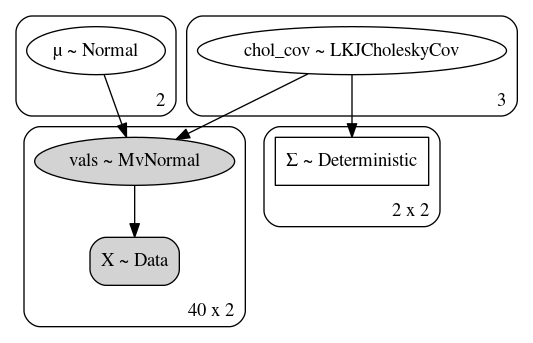
\includegraphics[width=\linewidth]{img/gen/pp_mvn_graph.png}
	\caption{Граф байесовской модели для оценки параметров многомерного нормального распределения. }
	\label{fig:pp_mvn_graph}
\end{figure}

Каждый <<трейс>> (набор цепей Маркова) в выводе алгоритма MCMC описывает апостериорное распределение рассматриваемых величин (параметров). На рис. \ref{fig:pp_mvn_trace} показаны трейсы для модели многомерного распределения описанной графом на рисунке \ref{fig:pp_mvn_graph}. Для эффективности требуется чтобы эти трейсы были скоординированы между цепями (т. е. они должны иметь одинаковые распределения) и чтобы точки внутри каждой цепи были максимально некоррелированы друг с другом \cite{stan_user_guide}. По статистикам (см. \nameref{appendix}) и графикам видно, что эти требования выполняются для данной модели.

\begin{figure}[H]
	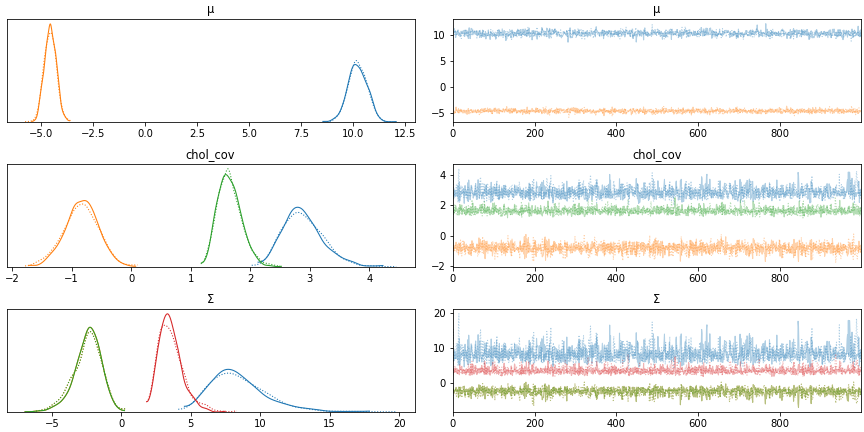
\includegraphics[width=\linewidth]{img/gen/pp_mvn_trace.png}
	\caption{Трейсы модели многомерного нормального распределения. }
	\label{fig:pp_mvn_trace}
\end{figure}

На рисунке \ref{fig:pp_mvn_mu_comparison} отображены гистограммы и оценки плотности распределения значений наблюдений $\mathbf{X} = D$, истинное значение параметра $\mu$, а также оценки значений методом максимального правдоподобия (MLE) и апостериорного среднего (posterior mean); для неинформативных априорных распределений эти оценки $\mu$ фактически совпадают. На рисунке \ref{fig:pp_mvn_mu_hdi} отображены апостериорные распределения средних значений и 95\%-е интервалы по сравнению с истинным значением. Такие же оценки (MLE, posterior mean) для матрицы ковариации можно увидеть на рисунке \ref{fig:pp_mvn_sigma_hdi}; легко заметить, что оценки максимального правдоподобия и максимум апостериори совпадают, а среднее значение апостериорного распределения смещено.

Таким образом проведено сравнение между классическими методами моделирования (максимального правдоподобия) и байесовскими методами вероятностного программирования (PP). Также подчеркнуты основные понятия и диаграммы PP, которые используются далее в работе.

\begin{figure}[H]
	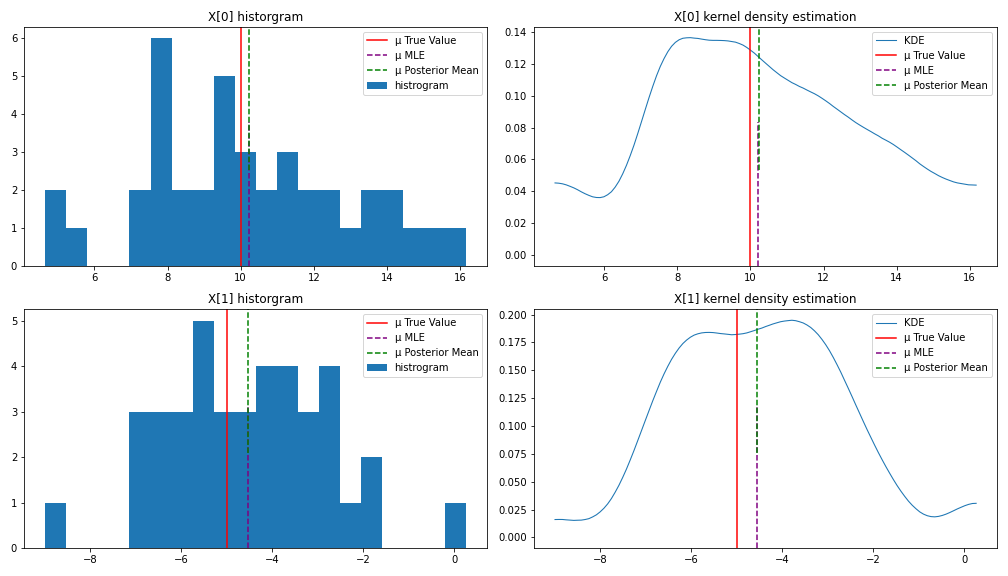
\includegraphics[width=\linewidth]{img/gen/pp_mvn_mu_comparison.png}
	\caption{Сравнения гистограммы данных с оценками $\mu$. KDE -- Kernel Density Estimation, метод локальной аппроксимации плотности. }
	\label{fig:pp_mvn_mu_comparison}
\end{figure}

\begin{figure}[H]
	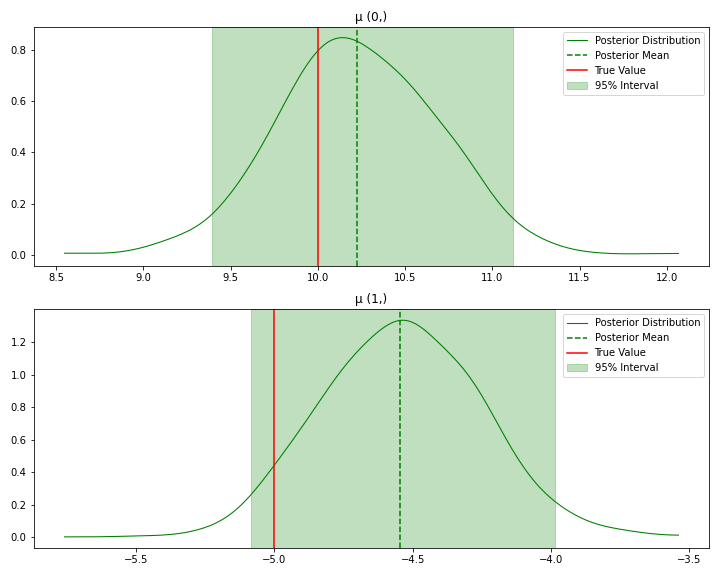
\includegraphics[width=\linewidth]{img/gen/pp_mvn_mu_hdi.png}
	\caption{Сравнение апостериорной оценки $\mu$ с известным значением. }
	\label{fig:pp_mvn_mu_hdi}
\end{figure}

\begin{figure}[H]
	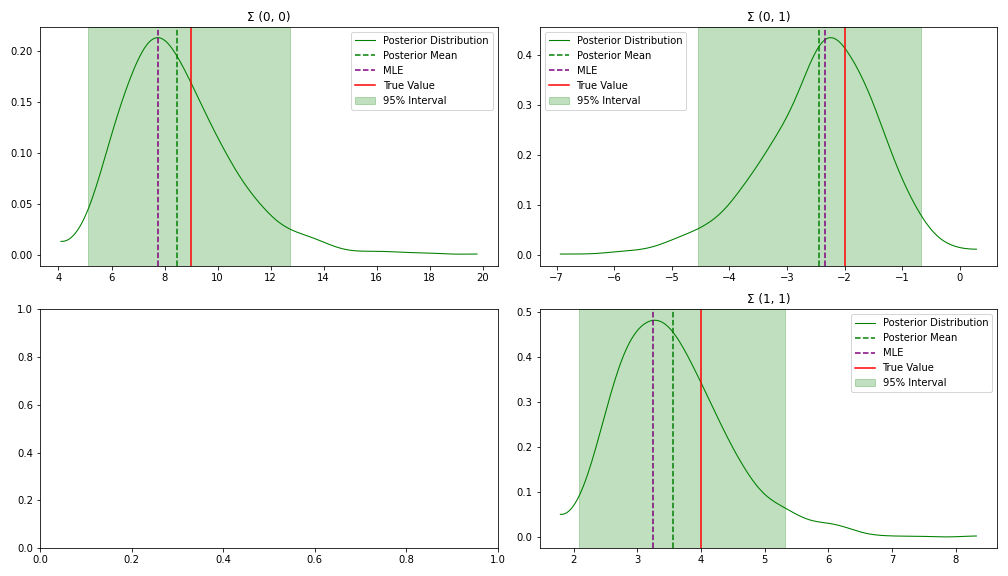
\includegraphics[width=\linewidth]{img/gen/pp_mvn_sigma_hdi.png}
	\caption{Сравнение апостериорной оценки $\Sigma$ с известным значением и оценкой максимального правдоподобия. }
	\label{fig:pp_mvn_sigma_hdi}
\end{figure}


\subsection{Модель векторной авторегресси (VAR)}

\label{subsection:var}

Для углубления в байесовское моделирование рассмотрим модель векторной авторегрессии размерности $n$ и порядка $p$ (т. е. $VAR(p)$, \textit{без} переключения), которая описывается уравнением \eqref{eq:pp_var_equation}:

\begin{equation}
	\begin{multlined}
		y_t = c + \sum\limits_{i=1}^{p}{A_{i}y_{t-i}} + \eta_t , 
		\quad
		\eta_t \sim N_n(0, \Sigma)
	\end{multlined}
	\label{eq:pp_var_equation}
\end{equation}

\noindent
где $y$ -- эндогенный вектор размерности $n$, $c$ -- векторная константа, $A_i, i\in\overline{1,p}$ -- $n \times n$ матрицы авторегрессионных коэффициентов, $\Sigma$ -- ковариационная матрица. Для коэффициентов $A_i$ должны выполнятся условия стационарности \cite{mal_multidim_nonhomogenous}. Также необходимо задать начальные значения ${y_{0}, y_{-1}, \dots, y_{-p+1}}$. 

В качестве примера рассмотрим сгенерированную выборку с известными параметрами. Для генерации рядов VAR используется библиотека \textit{regime\_switching}, разработанная автором (см. \nameref{appendix}). Создается случайный стационарный набор коэффициентов со следующими значениями (\textit{и соответствующими идентификаторами в программе}):

\begin{itemize}
	\item размерность (\textit{endog}) $n=2$ ;
	\item порядок (\textit{lag\_endog}) $p=1$ ;
	\item константа (\textit{coef\_const}) $c=[1.845, 0.8657]$ ;
	\item начальные значения (\textit{coef\_initial\_values}) $y_0=[2.134, 0.8573]$ ;
	\item матрица авторегрессионных коэффициентов (\textit{coef\_ar}) \\ $ A_1 = \begin{bmatrix} -0.3071 & 0.2489 \\ 0.4022 & -0.457 \end{bmatrix} $ ;
	\item ковариационная матрица (\textit{coef\_covariance}) \\ $ \Sigma = \begin{bmatrix} 0.8736 & -0.1628 \\ -0.1628 & 0.2488 \end{bmatrix} $ .
\end{itemize}

По этим параметрам генерируется одна реализация VAR процесса длиной $T=100$ (не включая начальные значения). Задача состоит в оценке всех параметров вероятностным программированием.

\begin{figure}[H]
	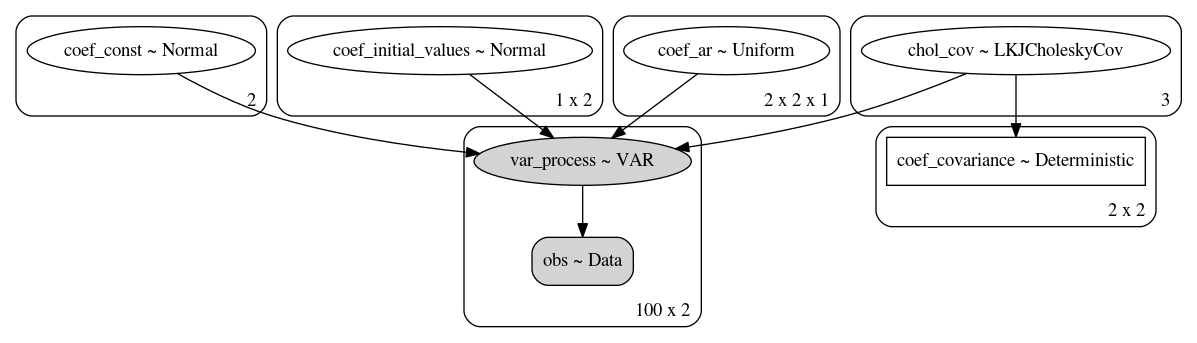
\includegraphics[width=\linewidth]{img/gen/pp_var_graph.png}
	\caption{Вероятностный граф для модели VAR. }
	\label{fig:pp_var_graph}
\end{figure}

На рисунке \ref{fig:pp_var_graph} изображен граф модели, схожий с предыдущей моделью. Для параметров используются неинформативные априорные распределения (большая дисперсия для нормальных и LKJ распределений \cite{lkj_prior}, равномерное распределение для коэффициентов авторегрессиронной матрицы); для деталей см. \nameref{appendix}. Вместо ``Normal'' для наблюдаемого процесса используется распределение ``VAR'' (с б\'{о}льшим количеством параметров); этот класс был реализован автором средствами библиотеки PyMC3. Для автоматического семплирования необходимо было определить только случайный генератор (для семплирования апостериорной плотности) и логарифмическую функцию правдоподобия \eqref{eq:pp_var_loglike}:

\begin{equation}
	\mathit{log}\mathcal{L}(c, A, \Sigma; \{y_t\})
	=
	\sum\limits_{t=1}^{T}{
	q(y_t - c - \sum_{i=1}^{p}{(A_i y_{t-i})}; 0, \Sigma)
	} ,
	\label{eq:pp_var_loglike}
\end{equation}

\noindent
где $q(\cdot; 0, \Sigma)$ -- функция логарифмического правдоподобия для многомерного нормального распределения с нулевым средним и дисперсией $\Sigma$.

На рис. \ref{fig:pp_var_trace} отображены трейсы (цепи MCMC и апостериорные распределения) для всех параметров. По вышеописанным критериям \cite{stan_user_guide} можно сделать вывод, что алгоритм сошелся и оценки параметров стабильны.

\begin{figure}[H]
	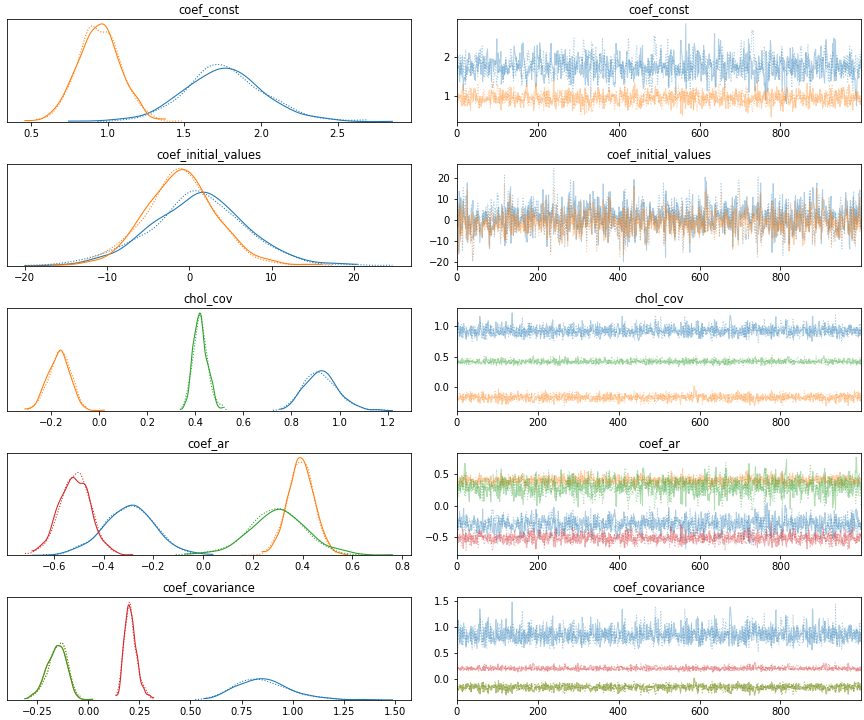
\includegraphics[width=\linewidth]{img/gen/pp_var_trace.png}
	\caption{Трейсы коэффициентов модели VAR}
	\label{fig:pp_var_trace}
\end{figure}

При сравнении коэффициентов (средние значения апостериорной плотности) в таблице \ref{tbl:pp_var_param_comparison} можно также увидеть сходство значений. Для начальных значений наблюдается большая неопределенность (это можно увидеть на рис. \ref{fig:pp_var_trace} для ``coef\_initial\_values''), но остальные коэффициенты близки к истинным значениями, и доверительные интервалы всех оценок включают истинные значения (см. \nameref{appendix} для дополнительных статистик).

\begin{table}[H]
	\begin{tabular}{ll|ll}
		\textbf{Параметр} & \textit{\textbf{(в коде)}} & \textbf{Оценка}              & \textbf{Истинное}            \\ \hline
		Константа         & \textit{coef\_const}       & $\begin{bmatrix} 1.76 & 0.944 \end{bmatrix}$ & $\begin{bmatrix} 1.85 & 0.866 \end{bmatrix}$ \\
		Нач. знач.        & \textit{coef\_initial}     & $\begin{bmatrix} 1.06 & -1.13 \end{bmatrix}$ & $\begin{bmatrix} 2.13 & 0.857 \end{bmatrix}$ \\
		Матрица AR        & \textit{coef\_ar}          & $\begin{bmatrix} -0.298 & 0.393 \\ 0.299 & -0.516 \end{bmatrix}$ & $\begin{bmatrix} -0.307 & 0.249 \\ 0.402 & -0.457 \end{bmatrix}$ \\
		Ковариация        & \textit{coef\_covar}       & $\begin{bmatrix} 0.860 & -0.153 \\ -0.153 & 0.208 \end{bmatrix}$ & $\begin{bmatrix} 0.874 & -0.163 \\ -0.163 & 0.259 \end{bmatrix}$ \\ \hline
	\end{tabular}
	\caption{Сравнение байесовских оценок и истинных значений параметров VAR. }
	\label{tbl:pp_var_param_comparison}
\end{table}


Для проверки адекватности модели также сравниваются апостериорное распределение одинаковых процессов с изначально наблюдаемым процессом \cite{stan_user_guide, arviz_2019}, как на рис. \ref{fig:pp_var_ppc}; видно, что модель с оцененными параметрами сможет сгенерировать наблюдаемые данные. Более наглядно это видно на \ref{fig:pp_var_realization}, где сравнивается наблюдаемая реализация с <<95\%-м корридором>> апостериорных симулированных реализаций. 

\begin{figure}[H]
	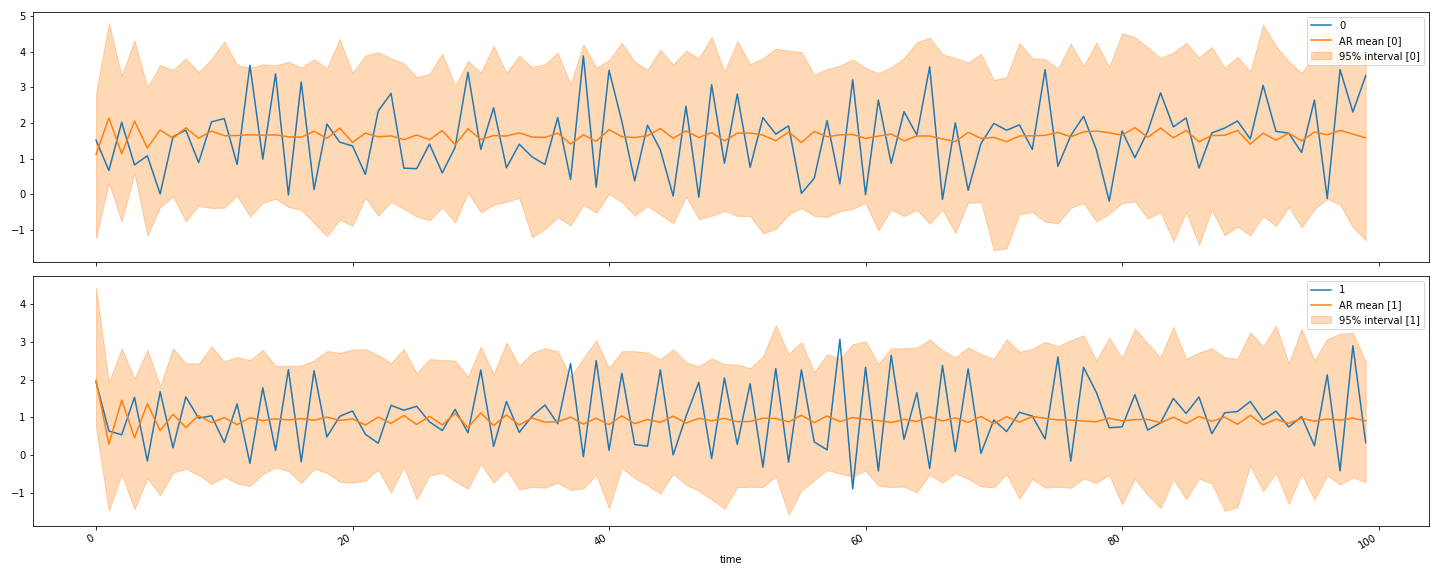
\includegraphics[width=\linewidth]{img/gen/pp_var_realization.png}
	\caption{Сравнение наблюденного процесса с апостериорным распределением VAR процессов (развернуто во времени). }
	\label{fig:pp_var_realization}
\end{figure}

\begin{figure}[H]
	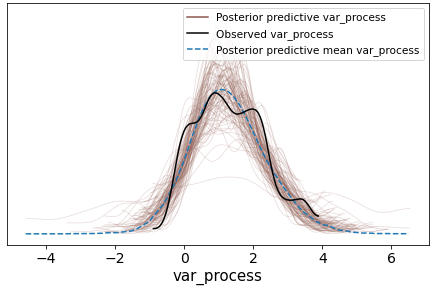
\includegraphics[width=\linewidth]{img/gen/pp_var_ppc.png}
	\caption{Сравнение наблюденного процесса с апостериорным распределением VAR процессов (одномерный график). }
	\label{fig:pp_var_ppc}
\end{figure}


\subsection{Распределение Пуассона с переключением параметра}

\label{subsection:ms_pois}

Далее рассмотрим задачу построения и оценивания RS-модели с помощью методов вероятностного программирования. Для определения графа модели необходимо определить случайные процессы $S$ и $F_l$ в параметризованном виде:

\begin{equation}
	l \sim S(\theta_S, \cdot) ,
\end{equation}

\begin{equation}
	y \sim F_l(\theta_{F(l)},\cdot) ,
\end{equation}

\noindent
где $\theta = (\theta_S, \theta_{F(1)}, \dots, \theta_{F(L)}) $ -- общий вектор параметров модели. 

Не обязательно чтобы эндогенный процесс $F(\cdot)$ RS-модели следовал (авто)регрессионной зависимости или даже непрерывному распределению. Для ознакомления с особенностями моделирования RS-моделей вероятностным программированием рассмотрим вариант переключения параметра пуассоновского распределения (без внешних зависимостей) на основании сгенерированных данных. Этот пример следует примеру, приведенному в \cite{blog_hidden_markov_ravinutala}; программный код и графики были доработаны автором.

Модель описывается переключением параметра $\lambda$ в пуассоновском распределении на основании значений цепи Маркова:

\begin{equation}
	\begin{aligned}
		y_t \sim \mathit{Pois}(\lambda_{l(t)}) , \\
		l_t \sim \mathit{Cat}(L, M_{l(t-1), \cdot}) .
	\end{aligned}
	\label{eq:ms_pois_equation}
\end{equation}

Такая модель может описывать, например, количество заявок, поступающих в систему за определенный промежуток времени; предполагается, что система может находиться в состоянии <<малой интенсивности>> или <<большой интенсивности>>. Была сгенерирована выборка длиной $T=100$ с числом классов $L=2$ и следующими параметрами:

\begin{equation}
	\lambda_1 = 5, 
	\lambda_2 = 10,
	M = \left[ {\begin{array}{cc}
					0.8 & 0.2 \\
					0.2 & 0.8
				\end{array} } \right]
	\label{eq:ms_pois_coef_true}
	.
\end{equation}

\noindent
По этим данным была построена следующая графовая модель, отображенная на рис. \ref{fig:pp_ms_pois_graph}:

\begin{figure}[H]
	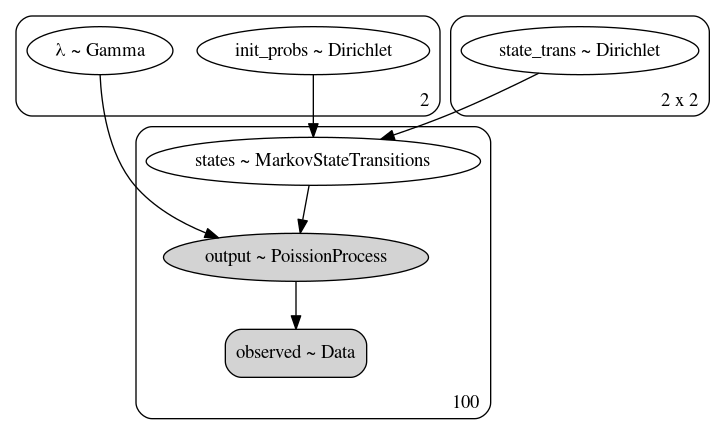
\includegraphics[width=\linewidth]{img/gen/pp_ms_pois_graph.png}
	\caption{Граф модели процесса с переключающимся пуассоновским распределением. }
	\label{fig:pp_ms_pois_graph}
\end{figure}

В качестве априорных распределений начальных состояний $\pi$ (на графе -- ``init\_probs’’) и матрицы перехода $M$ (на графе -- ``state\_trans’’) используется сопряженное распределение Дирихле с минимальной информативностью. Для $\lambda$ используется неинформативное Гамма\-распределение со среднем значением 10 и отклонением 100. Для процесса обозначенного ``states’’ достаточно было определить логарифмическую функцию правдоподобия, описанная формулой \eqref{eq:rs_loglike}:

\begin{equation}
	\mathit{log}\mathcal{L}(\pi, M; \{l_t\})
	=
	\mathit{log}\pi(l_1) + 
	\sum\limits_{t=2}^{T}{ 
	\mathit{log}\pi(l_t; l_{t-1}, \dots, l_1)
	} ,
	\label{eq:rs_loglike}
\end{equation}

\noindent
или, конкретно для цепи Маркова, формулой \eqref{eq:ms_loglike}:

\begin{equation}
	\mathit{log}\mathcal{L}(\pi, M; \{l_t\})
	=
	\mathit{log} \pi_{l(1)} + 
	\sum\limits_{t=2}^{T}{ 
	\mathit{log} M_{l(t); l(t-1)}
	} .
	\label{eq:ms_loglike}
\end{equation}

При работе с RS-моделями и алгоритмами MCMC наблюдается побочное явление ``label switching’’, т. е. переключение между режимами в середине цепи MCMC \cite{stan_user_guide,blog_hidden_markov_ravinutala}. Во время семплирования существует (например) некоторая вероятность спонтанной замены параметра режима 1 на параметр режима 2 и наоборот; в таком случае распределение дальнейших значений этих цепей будет отличаться от начального (т. к. они <<поменялись местами>>) и апостериорные значения параметров будут каким-то взвешенным среднем от исходных. Для простых моделей вроде этой, где есть достаточно четкая разделимость между классами, такое явление является редким: в процессе экспериментов переключение значения происходило только между целыми цепями. Для предотвращения явления ``label switching’’ в описанных моделях используется преобразование упорядочивания параметров \cite{blog_hidden_markov_ravinutala}.

На рис. \ref{fig:pp_ms_pois_trace} показаны результирующие трейсы, на рис.  \ref{fig:pp_ms_pois_ppc} -- график проверки апостериорных предсказаний модели, а на рис. \ref{fig:pp_ms_pois_fit} сравниваются предсказанные значения (эндогенную величину и класс состояния) с настоящими значениями. На графиках видно, что трейсы -- удовлетворительные, и апостериорные предсказания достаточно хорошо совпадают с истинными значения: полученные оценки коэффициентов \eqref{eq:ms_pois_coef_est} являются близкими к заданным в \eqref{eq:ms_pois_coef_true}. Оценки дисперсии и другие статистики представлены отдельно, см. \nameref{appendix}.

\begin{equation}
	\hat{\lambda}_1 = 4.703, 
	\hat{\lambda}_2 = 9.943,
	\hat{M}= \left[ {\begin{array}{cc}
					0.835 & 0.165 \\
					0.225 & 0.775
				\end{array} } \right]
	.
	\label{eq:ms_pois_coef_est}
\end{equation}

\begin{figure}[H]
	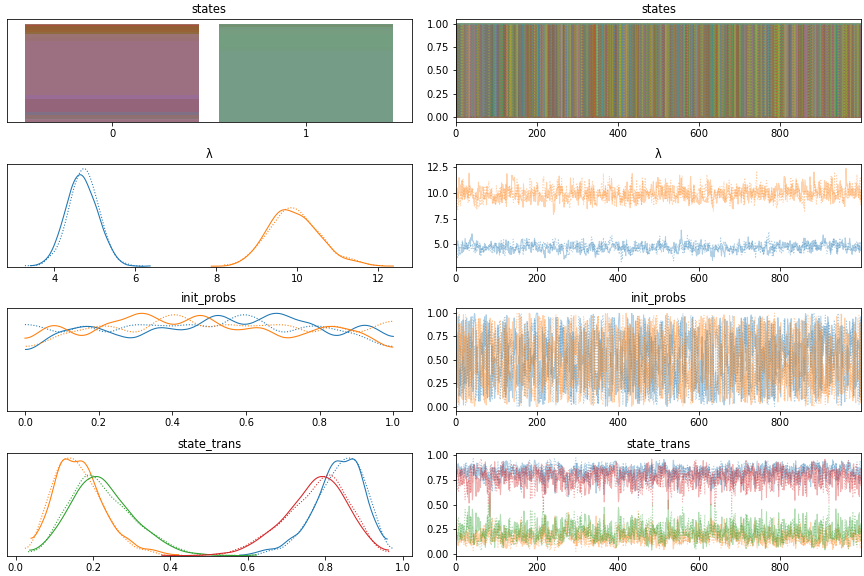
\includegraphics[width=\linewidth]{img/gen/pp_ms_pois_trace.png}
	\caption{Трейсы модели с пуассоновским переключением. }
	\label{fig:pp_ms_pois_trace}
\end{figure}

\begin{figure}[H]
	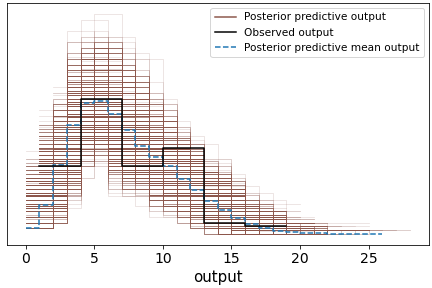
\includegraphics[width=\linewidth]{img/gen/pp_ms_pois_ppc.png}
	\caption{
		Диаграмма сравнения наблюдаемого процесса и апостериорных предсказаний модели \eqref{eq:ms_pois_equation}.
	}
	\label{fig:pp_ms_pois_ppc}
\end{figure}

\begin{figure}[H]
	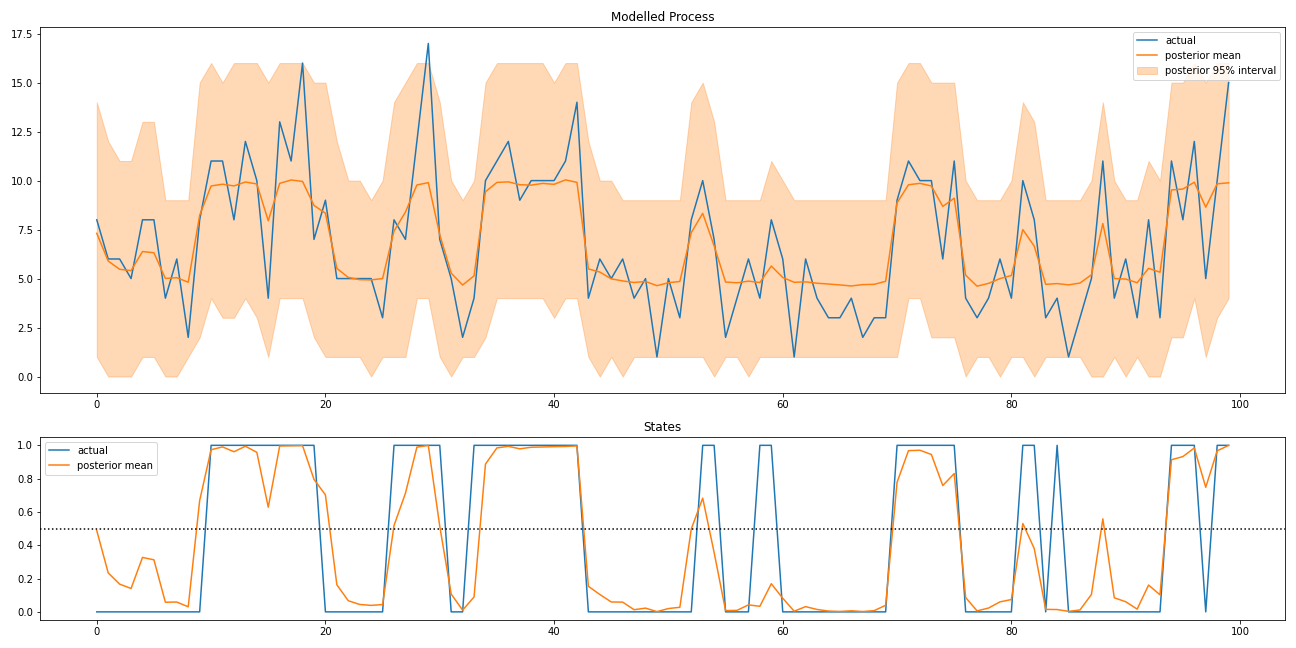
\includegraphics[width=\linewidth]{img/gen/pp_ms_pois_fit.png}
	\caption{Сравнение предсказаний и истинных значений модели \eqref{eq:ms_pois_equation}. \\
		Сверху: наблюдаемые значения, апостериорные оценки значений (среднее и 95\%-й интервал). \\
		Снизу: скрытые классы состояния (истинные и апостериорное среднее).
	}
	\label{fig:pp_ms_pois_fit}
\end{figure}

При смене предположении о процессе $S(\cdot)$ или $F(\cdot)$ не требуется построение другого алгоритма оценки; достаточно заменить соответствующий процесс. В главе \ref{chapter:msvarx_for_cycles} рассматривается процесс MS-ARX на реальных экономических данных; в реализации модели через вероятностное программирование необходимо переопределить только сам эндогенный процесс.


\chapter{Применение MS-VARX в задачах анализа бизнес-цикла экономики Республики Беларусь}

\label{chapter:msvarx_for_cycles}


\section{Экономические циклы и поворотные точки}

В рамках концепции экономического цикла или <<бизнес-цикла>> (business cycle), используемой в НБЭИ (Национальное бюро экономических исследований) США \cite{nberDevelopment}, подразумевается последовательная смена двух фаз базового экономического индикатора, называемых периодами <<роста>> (growth) и <<спада>> (recession) экономической активности \cite{oecdCycleExtraction}. Другие популярные определения экономических циклов могут состоять из трех или четырех фаз.

Моменты смены фазы роста на фазу спада, и наоборот, называются <<поворотными точками>> бизнес-цикла. Одной из ключевых задач анализа и прогнозирования экономической активности является разработка систем раннего обнаружения смены фаз экономических циклов.  Ранние работы \cite{esiMaking,esiExtra,mak_mal_bv_2018} рассматривали различные подходы оценивания поворотных точек для экономики Республики Беларусь. В качестве базового индикатора рассматривается реальное ВВП (GDP) Республики Беларусь.

В ходе НИР \cite{esiMaking} был построен композитный опережающий индикатор ESI (Economic Sentiment Index / Индекс Экономических Настроений / ИЭН). Для выделения циклических компонент ESI и GDP в работе был доработан метод, основанный на двойном применении фильтра Ходрика -- Прескотта. Из циклической компоненты ряда уже нетрудно получить оценки поворотных точек \cite{esiMaking,esiExtra}. 

У этого подхода есть ряд недостатков \cite{ham_never_hp}, самым главным который является невозможность прогнозирования рядов в будущее вследствие двусторонности фильтра Ходрика -- Прескотта. Автором была приведена альтернативная методика, основанная на использовании фильтра Хамильтона \cite{mak_mal_bv_2018}, которая исправляет часть недостатков.

Существует ешё один альтернативный подход оценивания поворотных точек, основанный на моделях с переключением состояний \cite{hamNewApproach}. В этой работе, в частности, используются авторегрессионные модели с переключением состояния и экзогенными переменными (класс MS-VARX) для которых разработаны алгоритмы оценивания параметров и классов состояния \cite{malNovopMSVARX,rs_persio2014,goutte_hal_00747479}. Каждое отдельное состояние $l$ интерпретируется как часть экономического цикла; например, при $L=2$, эти два класса интерпретируются как фазы роста и спада. 

Представленные ниже результаты основаны на недавней работе автора \cite{mak_mal_bv_2020} а так же дополнительных исследованиях этой задачи байесовскими методами.


\section{Описание исходных данных}

\label{section:gdp_data}

В качестве базового индикатора бизнес-цикла рассматривается реальный ВВП (GDP) Республики Беларусь в ценах 2014 г. в месячном исчислении; он же является моделируемой переменной. Вышеописанный Индекс Экономических Настроений (ESI) используется в качестве экзогенной переменной. Так как ESI является опережающим индикатором (поворотные точки ESI опережают поворотные точки GDP на 2-4 месяца \cite{esiMaking,esiExtra}), рассматривались варианты моделей со включением различных лагов ESI (рассматривались варианты опережения от 0 до 5 периодов). 

Цель экспериментальной части \cite{mak_mal_bv_2020} состоит в оценивании предиктивных способностей моделей MS-ARX, включающих вышеописанный опережающий индикатор. Ряды GDP и ESI содержат сезонные эффекты. В представляеных моделях использовались годовые темпы ростов этих рядов (GGDP и GESI соответственно), которые можно рассматривать как сезонно скорректированные ряды. Их циклические компоненты демонстрируют опережающий характер GESI\_C по отношению к GGDP\_C \cite{mak_mal_bv_2020}, см. рис. \ref{fig:ggdp_gesi_cycles}. Во всех моделях используются 121-125 наблюдений GGDP и GESI (период 2007-2017 гг.).

\begin{figure}[H]
	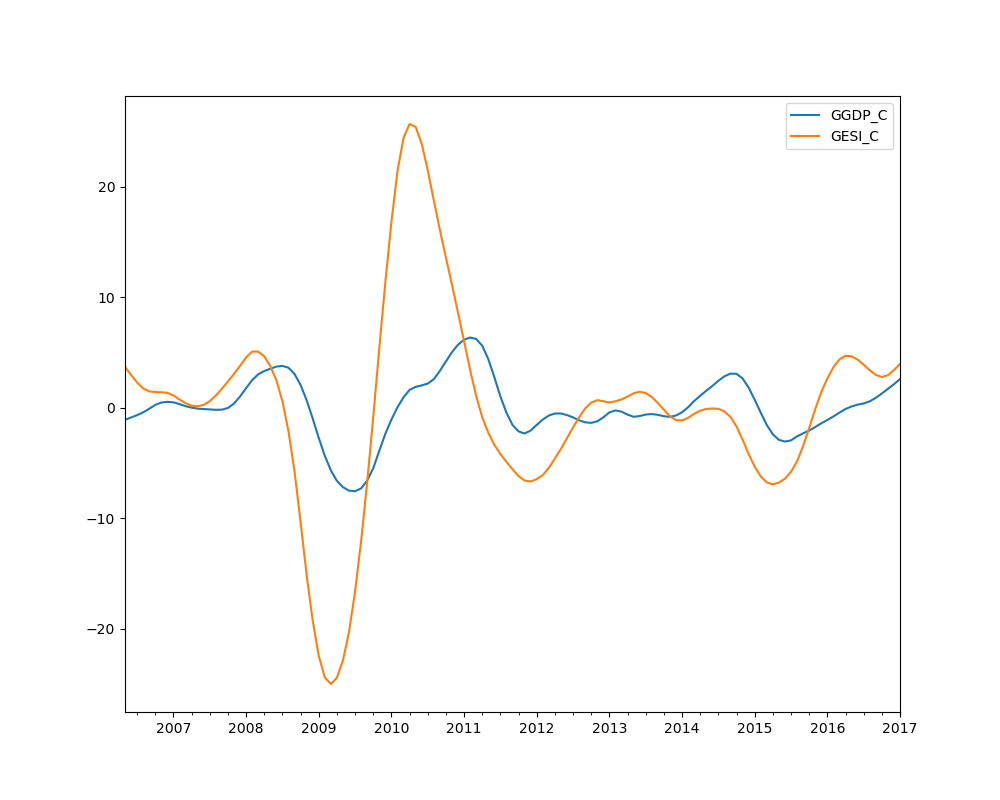
\includegraphics[width=\linewidth]{img/manual/ggdp_gesi_cycles.png}
	\caption{Циклы годовых темпов роста ВВП (GGDP) и ИЭН (GESI), полученные по методике \cite{esiMaking}. }
	\label{fig:ggdp_gesi_cycles}
\end{figure}


\section{Исследование рядов GGDP, GESI статистическими тестами}

\label{section:gdp_stattests}

Для тестирования интегрированности рядов GGDP и GESI (и их первых разностей) использовались тесты, допускающие наличие структурных изменений. Используя тест BPUR (Breakpoint Unit Root), гипотеза об интегрированности с <<инновационными аномалиями>> (сдвигами) не была отклонена. 
С помощью теста Баи – Перрона (Bai – Perron tests for sequentially determined breaks) и построения моделей со структурными изменениями (Breakpoint Least Squares) выявлен феномен <<кобрейкинга>> (одновременного структурного изменения) рядов GGDP и GESI. 
Более подробно процедура описана в \cite{mak_mal_bv_2020}, где также построены две ARX модели (формулы 4 и 5 в статье), не включающие изменения в параметрах т. к.  структурные изменения в GGDP и GESI совпадают. Также было проведено тестирование на коинтегрированность этих рядов, в котором гипотеза о коинтеграции не была отклонена \cite{mak_mal_bv_2020}. 

Принятая методология определения фаз бизнес-цикла экономики Республики Беларусь предполагает две фазы (<<спад>> и <<подъем>>), поэтому фиксируется количество классов $L=2$, которые интерпретируются соответствующим образом. В данной работе везде использовался класс моделей MS-ARX в продолжение серии работ автора и руководителя по данной тематике \cite{mak_mal_bv_2018,malVARforCycles}.


\section{Эксперименты с MS-ARX и опережающим индикатором}

При моделировании GGDP рассматривались некоторые модели семейства MS-ARX, включающие различные структурные предположения и экзогенные переменные \cite{mak_mal_bv_2020}. Везде рассматривались $L=2$ класса и порядок авторегрессии не превышающий $p=2$, т. е. класс MS(2)-ARX(2). В дальнейших формулах используются обозначения $y_t = \text{GGDP}_t$, \: $x_t = \text{GESI}_t$ и $\eta_t$ -- инновационный процесс.

Для данного этапа моделирования использовались классические методы с помощью библиотеки Statsmodels \cite{statsmodels}. Из рассмотренных моделей \cite{mak_mal_bv_2020}, наилучшие результаты были получены в приведенных ниже $M.0$ -- $M.3$.

\begin{equation}
	M.0. \quad y_t = c_{l(t)} + \alpha_{l(t), 1} y_{t-1} + \alpha_{l(t), 2} y_{t-2} + \eta_t .
\end{equation}

Модель $M.0$ не содержит экзогенных факторов и предполагает, что циклические изменения обусловлены аномалиями в инновационном процессе $\eta$ и ведут к изменениям среднего уровня GGDP.

\begin{figure}[H]
	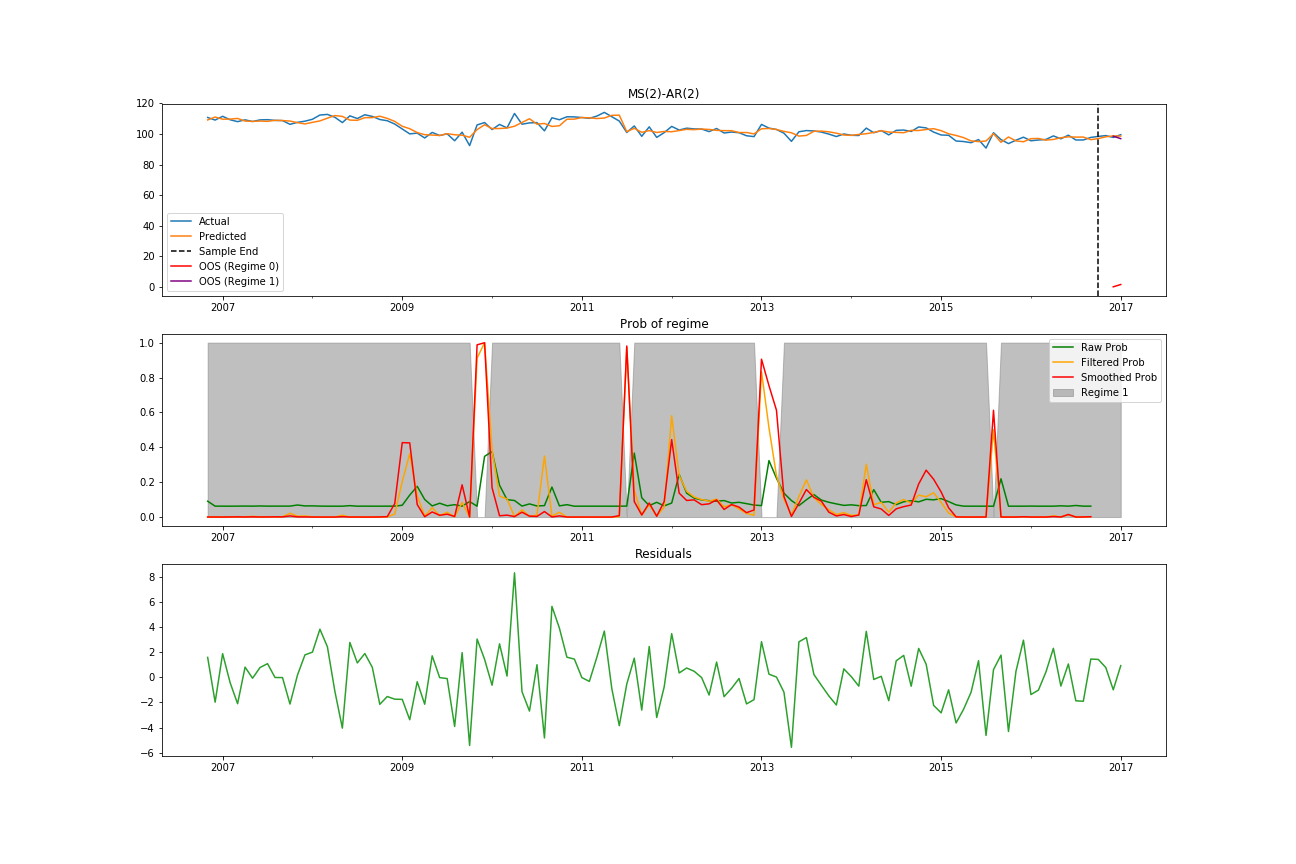
\includegraphics[width=\linewidth]{img/manual/model_m0.png}
	\caption{
		Результаты модели $M.0$: предсказание эндогенной переменной (верхняя панель), вероятности режимов (средняя панель), остатки модели (нижняя панель).
	}
	\label{fig:sm_model_m0}
\end{figure}

Для моделей $M.1$ -- $M.3$ отключено изменение в авторегрессионных коэффициентах $\alpha_i$; вследствие выявленной незначимости этих коэффициентов они были исключены в итоговых вариантах моделей.

\begin{equation}	
	M.1. \quad y_t = c_{l(t)} + \alpha_1 y_{t-1} + \alpha_2 y_{t-2} + \beta_{l(t), 1} t + \eta_t .
\end{equation}

Модель $M.1$ допускает циклические изменения в трендовой компоненте. 

\begin{figure}[H]
	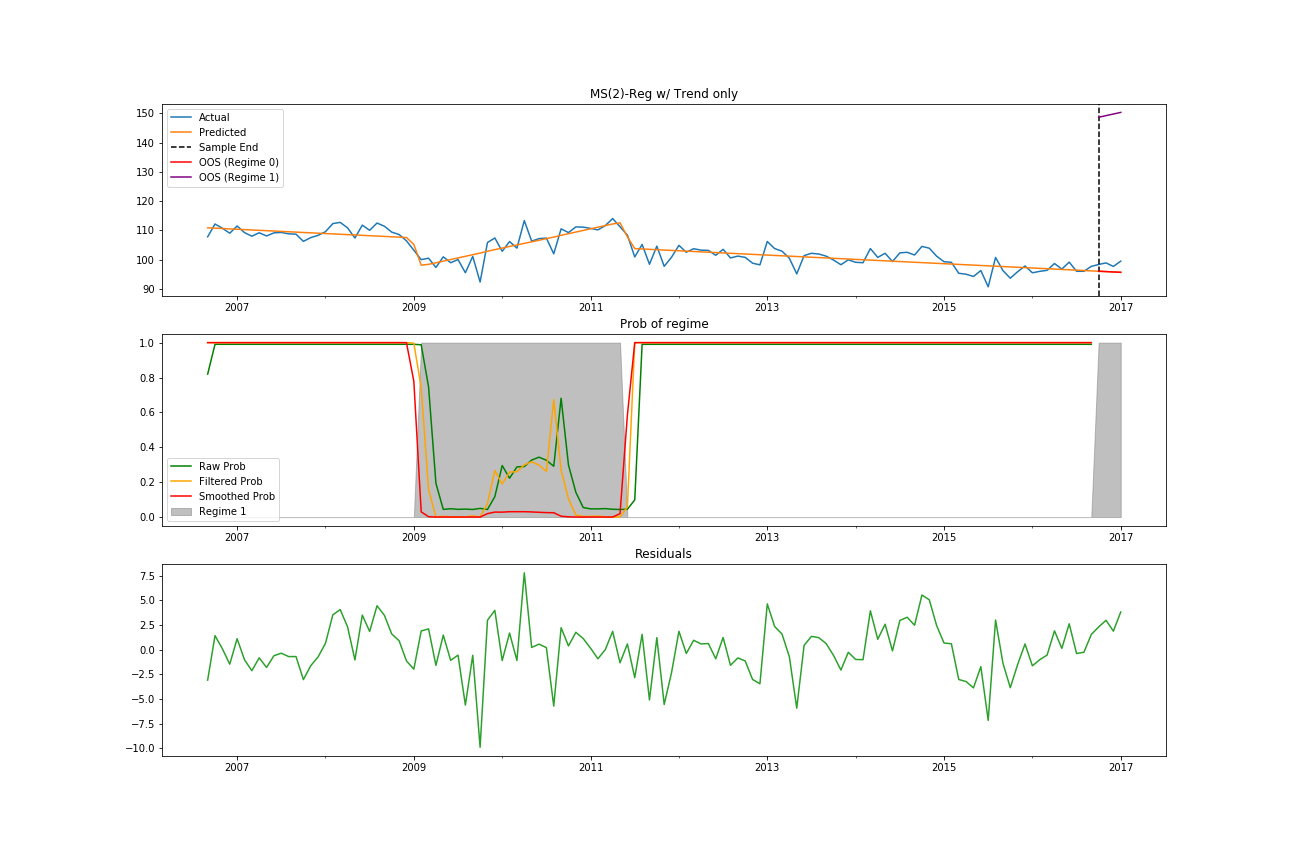
\includegraphics[width=\linewidth]{img/manual/model_m1.png}
	\caption{
		Результаты модели $M.1$: предсказание эндогенной переменной (верхняя панель), вероятности режимов (средняя панель), остатки модели (нижняя панель).
	}
	\label{fig:sm_model_m1}
\end{figure}

В основе $M.2$ лежит долгосрочная коинтеграционная зависимость между GGDP и GESI, включающая линейный тренд:

\begin{equation}
	M.2. \quad y_t = c_{l(t)} + \alpha_1 y_{t-1} + \alpha_2 y_{t-2} + \beta_{l(t), 1} t + \beta_{l(t), 2} x_{t} + \eta_t .
\end{equation}

\begin{figure}[H]
	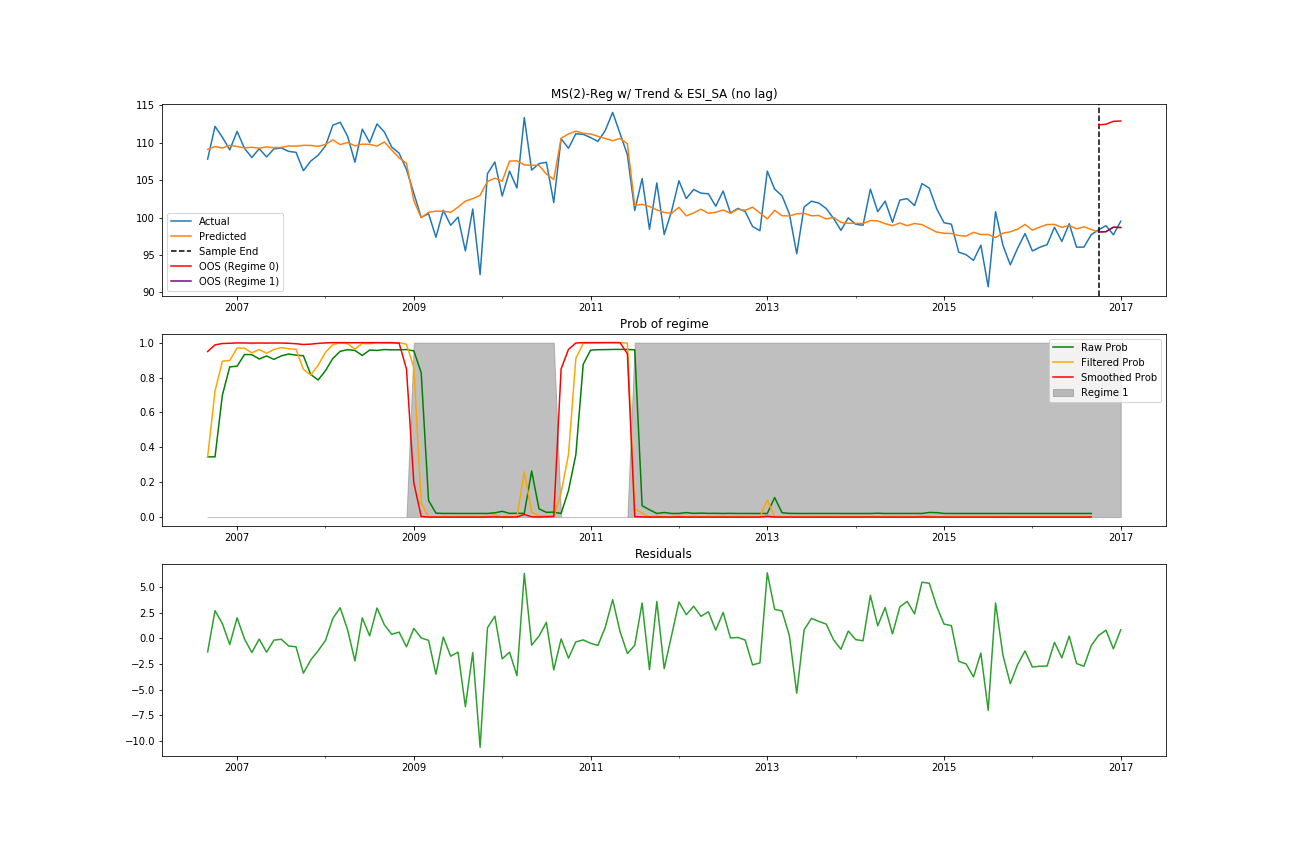
\includegraphics[width=\linewidth]{img/manual/model_m2.png}
	\caption{
		Результаты модели $M.2$: предсказание эндогенной переменной (верхняя панель), вероятности режимов (средняя панель), остатки модели (нижняя панель).
	}
	\label{fig:sm_model_m2}
\end{figure}

Модель $M.3$ использует такую же структуру, как и $M.2$, однако включает экзогенную переменную GESI[-4] как опережающую:

\begin{equation}
	M.3. \quad y_t = c_{l(t)} + \alpha_1 y_{t-1} + \alpha_2 y_{t-2} + \beta_{l(t), 1} t + \beta_{l(t), 2} x_{t-4} + \eta_t .
	\label{eq:ms_arx_m3}
\end{equation}

\begin{figure}[H]
	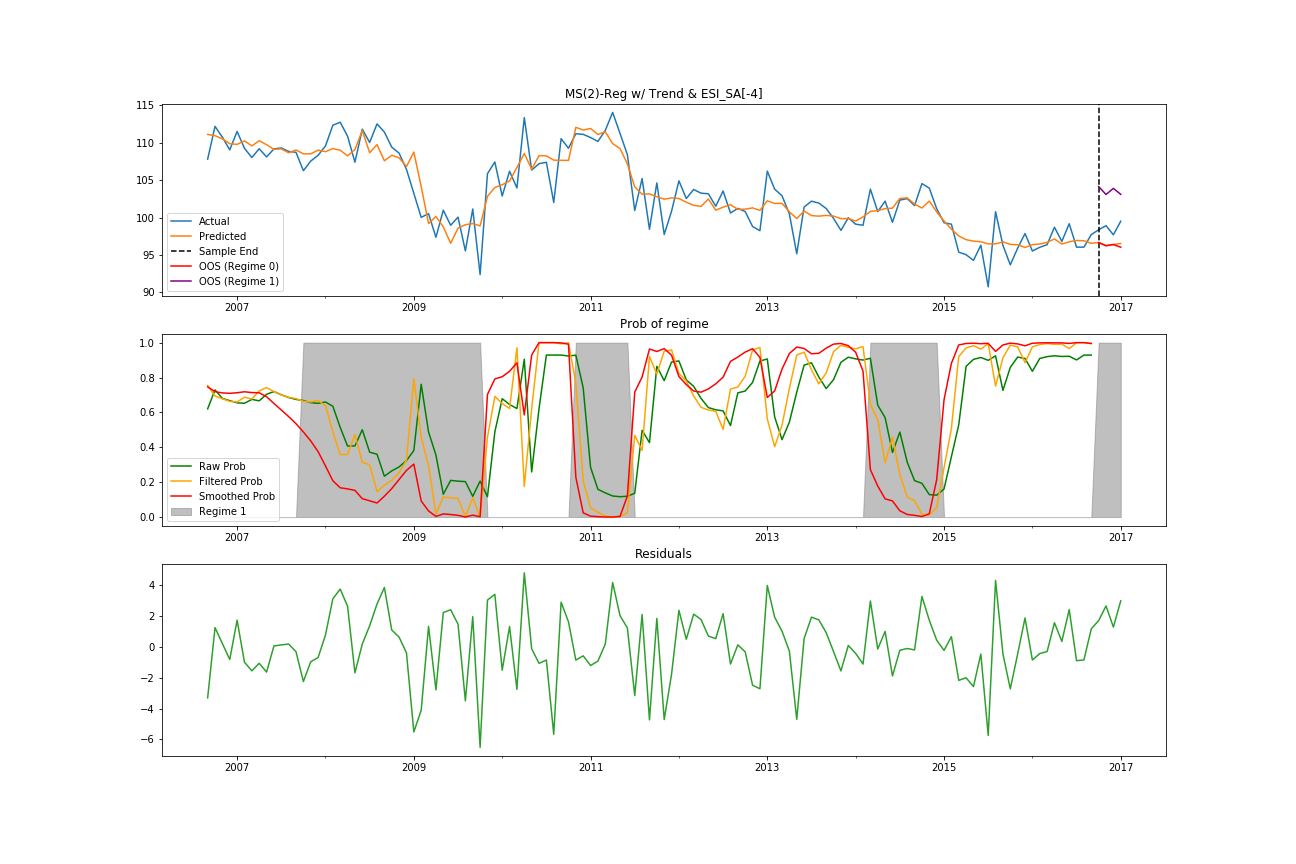
\includegraphics[width=\linewidth]{img/manual/model_m3.png}
	\caption{
		Результаты модели $M.3$: предсказание эндогенной переменной (верхняя панель), вероятности режимов (средняя панель), остатки модели (нижняя панель).
	}
	\label{fig:sm_model_m3}
\end{figure}

Все коэффициенты при экзогенных переменных зависят от класса состояния $l_t$.

Графическое представление результатов экспериментов приведено на рисунках \ref{fig:sm_model_m0}, \ref{fig:sm_model_m1}, \ref{fig:sm_model_m2} и \ref{fig:sm_model_m3}. На каждом графике представлены:
\begin{itemize}
	\item динамика годовых темпов роста реального ВВП (GGDP);
	\item интервалы, соответствующие классам <<роста>> и <<спада>>;
	\item прогнозы моделей для периода оценивания (обучения) модели;
	\item условные прогнозы моделей вне этого периода (для валидации);
	\item график оценок вероятности режима 1 (raw -- прямая оценка, filtered -- условная вероятность по предыдущим значениям, smoothed -- условная вероятность по всем значениям);
	\item график остатков.
\end{itemize}

В таблицах \ref{tbl:ggdp_model_params_reg} и \ref{tbl:ggdp_model_params_ms} приведены характеристики оцененных моделей, включая коэффициенты, интерпретацию фаз <<роста>> и <<падения>>, и вероятности переходов. На основании этих данных можно сделать следующие выводы:

\begin{enumerate}
	\item Свободный член и экзогенные переменные, включенные в модели, действительно подвержены циклическим изменениям во всех выделеных моделях.
	\item В моделях $M.0$, $M.1$, $M.2$ в состоянии <<спад>> GGDP чувствительна к изменениям в свободном члене и всех включенных переменных (тренд, GESI, авторегрессионная часть), а в состоянии <<рост>> влияние оказывает только свободный член.
	\item В модели $M.3$ с опережающей переменной GESI[-4] все коэффициенты значимые, и сама модель обладает наилучшей предиктивной способностью при определении двух классов состояния.
\end{enumerate}

\begin{table}[H]
	\begin{tabular}{l|ll|ll}
		\hline
		\multicolumn{1}{c|}{\multirow{2}{*}{\textbf{Модель}}} & \multicolumn{1}{c}{\multirow{2}{*}{\textbf{Переменная}}} & \multicolumn{1}{c|}{\multirow{2}{*}{\textbf{Параметр}}} & \multicolumn{2}{c}{\textbf{Значение / p-статистика}}                                     \\
		\multicolumn{1}{c|}{}                                 & \multicolumn{1}{c}{}                                     & \multicolumn{1}{c|}{}                                   & \multicolumn{1}{c}{Фаза <<спад>>}                    & \multicolumn{1}{c}{Фаза <<рост>>} \\ \hline
		\multirow{3}{*}{$M.0$}                                & -                                                        & $c$                                                     & 100,7035/0,000                                       & 103,5599/0,000                    \\
		                                                      & GGDP[-1]                                                 & $\alpha_1$                                              & 0,4036/0,000                                         & 0,0829/0,743                      \\
		                                                      & GGDP[-2]                                                 & $\alpha_2$                                              & 0,5533/0,000                                         & -0,2713/0,178                     \\ \hline
		\multirow{2}{*}{$M.1$}                                & -                                                        & $c$                                                     & 104,3309/0,000                                       & 109,4102/0,000                    \\
		                                                      & t                                                        & $\beta_1$                                               & -0,0536/0,000                                        & 0,0050/0,840                      \\ \hline
		\multirow{3}{*}{$M.2$}                                & -                                                        & $c$                                                     & 92,415/0,000                                         & 101,6467/0,000                    \\
		                                                      & t                                                        & $\beta_1$                                               & -0,0690/0,000                                        & 0,0256/0,289                      \\
		                                                      & GESI                                                     & $\beta_2$                                               & 0,1373/0,000                                         & 0,0750/0,254                      \\ \hline
		\multirow{3}{*}{M.3}                                  & -                                                        & $c$                                                     & 73,7080/0,000                                        & 98,919/0,000                      \\
		                                                      & t                                                        & $\beta_1$                                               & -0,0622/0,000                                        & -0,1169/0,000                     \\
		                                                      & GESI[-4]                                                 & $\beta_2$                                               & 0,3569/0,000                                         & 0,1118/0,000                      \\ \hline
	\end{tabular}
	\caption{Сравнение регресионных параметров MS моделей. }
	\label{tbl:ggdp_model_params_reg}
\end{table}

\begin{table}[H]
	\begin{tabular}{l|ll|ll|ll}
		\hline
		\multicolumn{1}{c|}{\textbf{Модель}} & \multicolumn{1}{c}{$\hat{M}_{0,0}$ / p-стат.} & \multicolumn{1}{c|}{$\hat{M}_{0,1}$} & \multicolumn{1}{c}{$\hat{M}_{1,0}$ / p-стат.} & \multicolumn{1}{c|}{$\hat{M}_{1,1}$} & \multicolumn{1}{c}{$\hat{\pi}_0$} & \multicolumn{1}{c}{$\hat{\pi}_1$} \\ \hline
		$M.1$                                & 0,9784/0,000                                  & 0,0216                               & 0,3430/0,204                                  & 0,6570                               & 0,614                             & 0,386                             \\
		$M.2$                                & 0,9611/0,000                                  & 0,0389                               & 0,2050/0,172                                  & 0,7950                               & 0,655                             & 0,345                             \\
		$M.3$                                & 0,9288/0,000                                  & 0,0712                               & 0,1163/0,124                                  & 0,8837                               & 0,620                             & 0,380                             \\ \hline
	\end{tabular}
	\caption{Сравнение параметров состояний MS моделей. }
	\label{tbl:ggdp_model_params_ms}
\end{table}


\section{MS-ARX в парадигме вероятностного программирования}

\label{section:msarx_pp}

Повторим процесс построения наилучшей модели $M.3$ (формула \eqref{eq:ms_arx_m3}) 
\footnote{Значения вероятности классов модели $M.3$ зависит от начальных условий EM-алгоритма, поэтому для этой части работы значения могут отличаться от предыдущей. В новой итерации все значения случайных параметров фиксированы, см. \nameref{appendix}. }
, но используя байесовский подход и вероятностное программирование. 

Как и в случаях моделей VAR и MS-Pois, в библиотеке PyMC3 отсутствует готовый класс для MS-ARX или даже MS-MLR (регрессии с переключением). Был построен байесовский граф модели, который изображен на рис. \ref{fig:pp_ms_arx_graph_man} \footnote{Расположение элементов графа поправлены в интересах читаемости}. В качестве априорных распределений коэффициентов взяты неиформативные (широкие) распределения, как описано ранее в части \ref{subsection:mvn}.

Класс ``MarkovStateTransitions'' в этой модели переиспользован из части \ref{subsection:ms_pois} (см. рис. \ref{fig:pp_ms_pois_graph}). 
Класс ``SwitchingRegression2'' был разработан автором с учетом феномена ``label switching'', описанного в части \ref{subsection:ms_pois}. Предотвращать переключение многомерных коэффициентов нетривиально. Было принято решение использовать упорядочивание по среднему значению условного среднего по всем наблюдениями, т.е. среднее узла ``conditional mean'' на графе по наблюдениям.
На графе также изображены значения состояний ``sm\_states'' (оценки значений классов, полученные классическими методами), однако при обучении байесовский модели они используются лишь в качестве начальных точек (тестовых значений) траекторий MCMC.

\begin{figure}[H]
	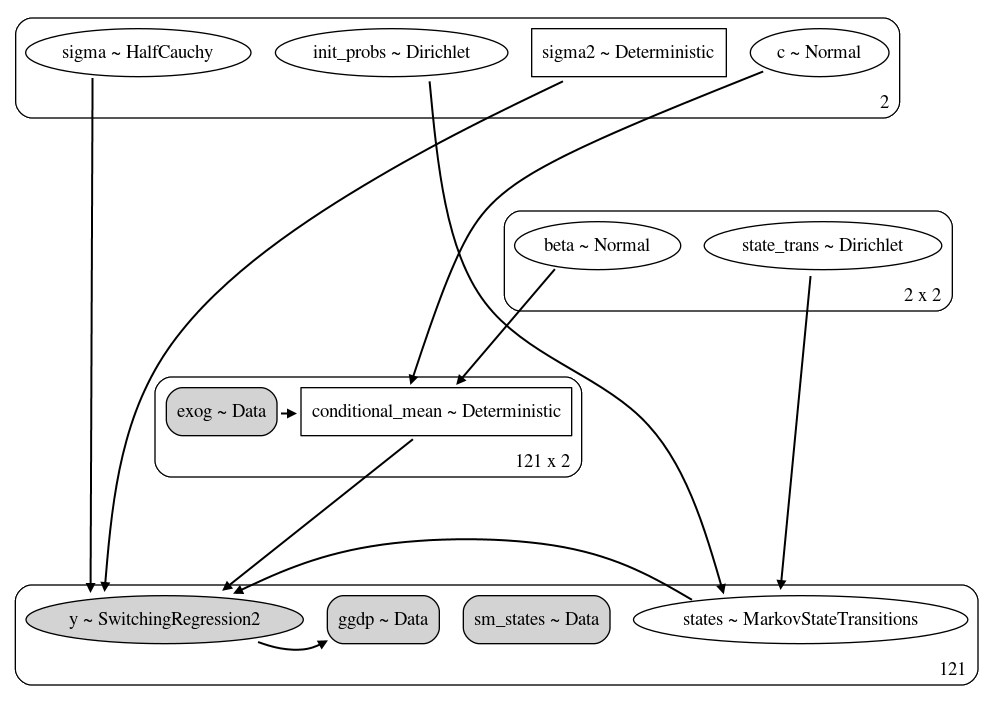
\includegraphics[width=\linewidth]{img/manual/pp_ms_arx_graph_man.png}
	\caption{Байесовский граф модели MS-MLR. }
	\label{fig:pp_ms_arx_graph_man}
\end{figure}


\begin{figure}[H]
	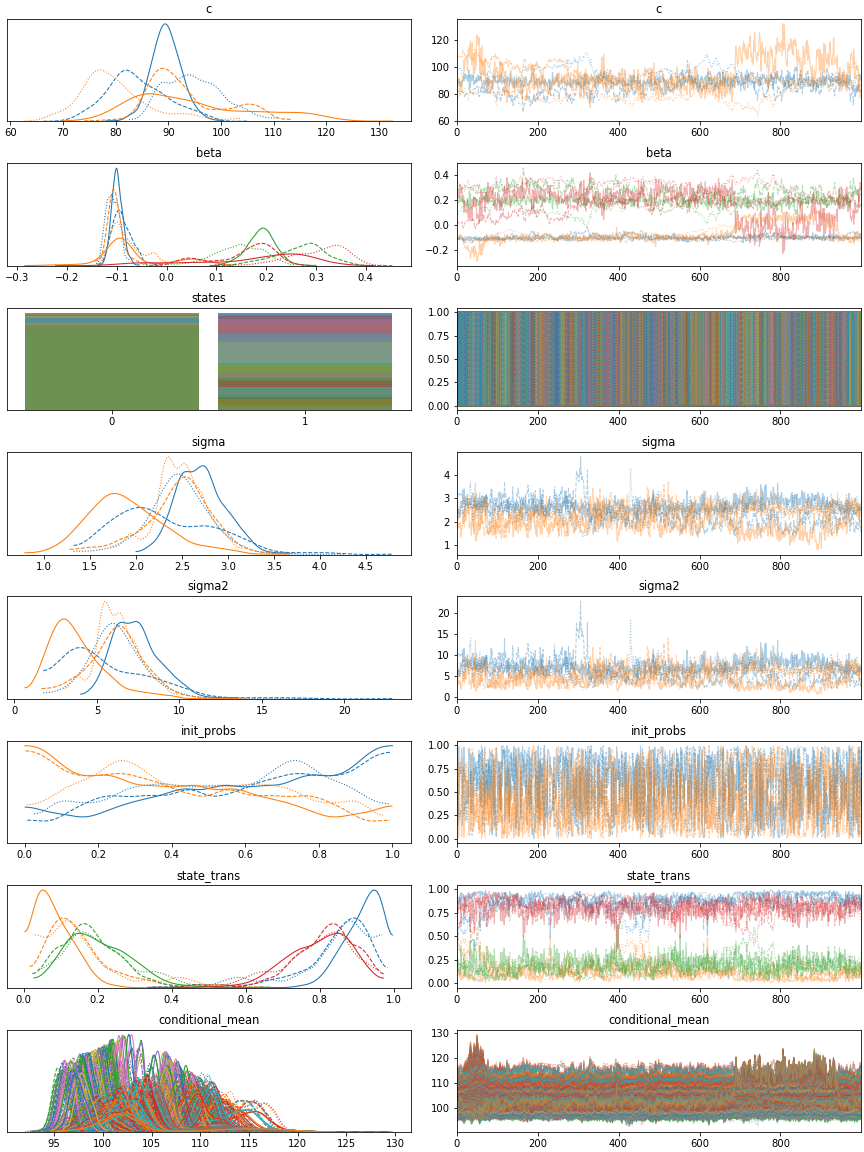
\includegraphics[width=\linewidth]{img/gen/pp_ms_arx_trace.png}
	\caption{Трейсы для модели MS-MLR. }
	\label{fig:pp_ms_arx_trace}
\end{figure}

Библиотекой PyMC3 автоматически выбирались алгоритмы NUTS \cite{nuts_hoffman_gelman} для неприрывных параметров и Binary Gibbs-Metropolis \cite{pymc3_2016} для классов состояния. Этими алгоритмами были получены трейсы, отображенные на рис. \ref{fig:pp_ms_arx_trace}. Ссылаясь на критерии описанные раннее в части \ref{subsection:mvn} \cite{stan_user_guide}, можно увидеть, что трейсы не вполне удовлетворительные:

\begin{enumerate}
	\item В некоторых случаях не удалось избежать скачкообразного изменения параметров; это четко видно на 700-м шаге цепей для $c$, $\beta$.
	\item Для параметра $\sigma^2$ также происходит ``label switching''; видно, что распределения разных цепей меняются местами.
	\item Апостериорные распределения также не полностью согласуются по цепям. Об этом так же свидетельствуют значения статистики $\hat{R} > 1.4$, о чем автоматически предупреждает PyMC3 \cite{pymc3_2016,nuts_hoffman_gelman}.
\end{enumerate}

Проделанные автором улучшения не смогли полностью преодолеть проблему ``label switching''. Вследствие этого, средние апостериорные значения коэффициентов более близки друг к другу чем для оценок EM-алгоритмом (см. \nameref{appendix}). Работа над устранение этой проблемы продолжается. 

Однако, несмотря на вышеописанные проблемы, результаты предсказаний значений близки к истинным, и предсказанные классы (даже вероятности) близко следуют вероятностям, полученным классическими статистическими методами \footnote{В данном случаи, библиотекой Statsmodels \cite{statsmodels}. }. Сравнение приведено на рис. \ref{fig:pp_ms_arx_fit}.

Остатки модели (см. рис. \ref{fig:pp_ms_arx_resid}) некоррелированы и близки к нормальным, с выбросами в положительную сторону в течении периода 35-50 \footnote{Этот период соответствует экономическому кризису 2009-2010 гг. в Республики Беларусь. }. В целом, модель хорошо описывает данные и признана автором удовлетворительной, несмотря на сомнительную стабильность трейсов.

\begin{figure}[H]
	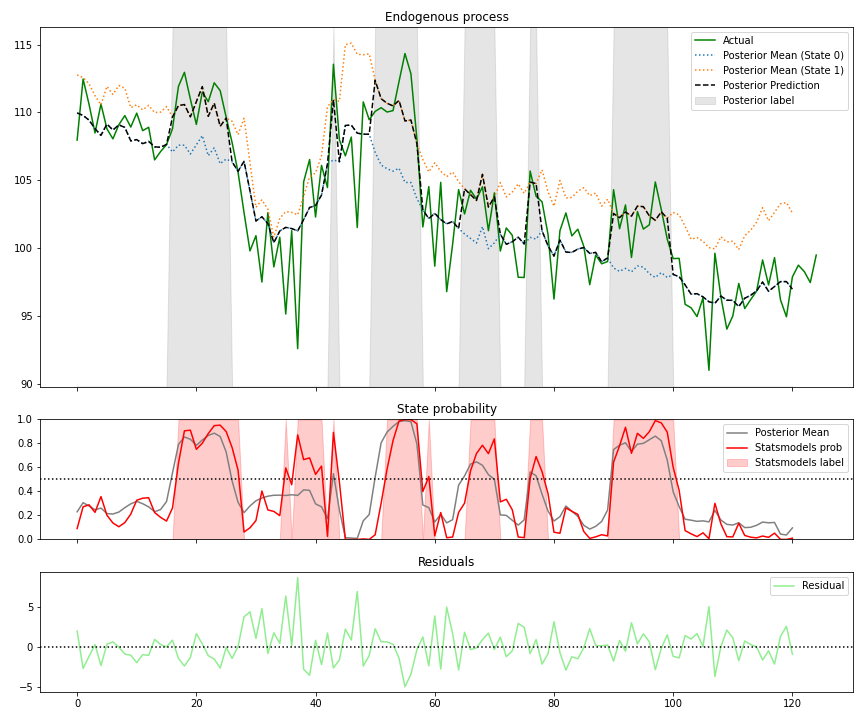
\includegraphics[width=\linewidth]{img/gen/pp_ms_arx_fit.png}
	\caption{
		Сравнение предсказанных значений эндогенной переменной и класса состояния. \\
		Верхняя панель: сравнение средних обоих классов с наблюдениями. \\
		Средняя панель: сравнение вероятностей классов классического и байесовского подхода. \\
		Нижняя панель: ряд остатков модели.
	}
	\label{fig:pp_ms_arx_fit}
\end{figure}


\begin{figure}[H]
	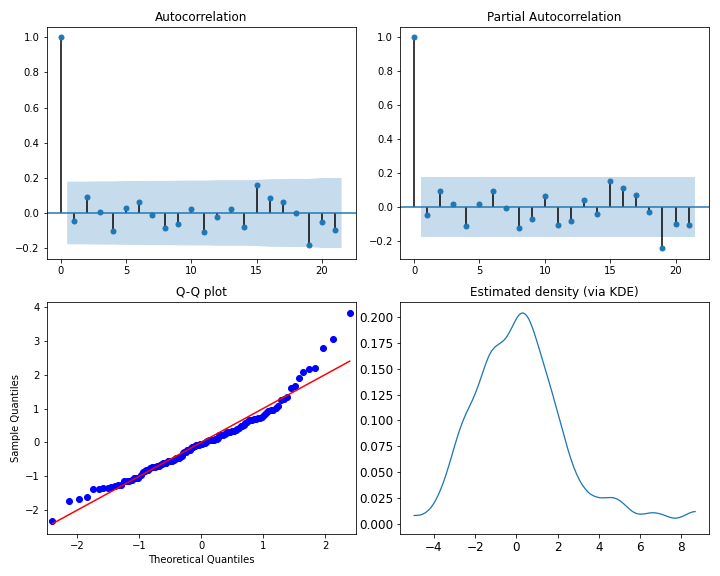
\includegraphics[width=\linewidth]{img/gen/pp_ms_arx_resid.png}
	\caption{
		Исследование остатков байесовской модели: 
		проверки на автокорреляцию и нормальность.
	}
	\label{fig:pp_ms_arx_resid}
\end{figure}


% Заключение (выводы)
\fakechapter{Заключение}

% В «Заключении» формулируются основные результаты исследования и практические рекомендации по их использованию. 
% Выводы формулируются по пунктам и излагаются последовательно по каждому разделу магистерской диссертации. Выводы должны быть конкретными и обоснованными, вытекать из содержания магистерской диссертации. 

Методы анализа данных, использующие скрытые состояния, все больше используются как в исследованиях, так и на практике. Класс моделей с переключением состояния (RS-модели) является относительно простым, но важным подклассом моделей с латентными переменными, которые находят применение во многих областях. 

В данной магистерской работе проводится многостороннее исследование RS-моделей: методами классической статистики и вероятностным программированием, на сгенерированных данных и на реальных данных экономики Республики Беларусь. 

В первой главе работы приведен последовательный обзор теории общих RS-моделей, моделей IS-VARX и MS-VARX, и итерационного EM-алгоритма совместной оценки параметров и классов состояния. Вторая глава вводит основные понятия байесовских графовых моделей и вероятностного программирования. На основании последующих примеров моделей рассматриваются детали работы с алгоритмами MCMC, включая особенности применения к RS-моделям. Этот материал включает существенные доработки автора (имплементации байесовских моделей VAR и цепи Маркова в контексте пакета PyMC3).

Третья глава работы сфокусирована на практической задаче моделирования бизнес-цикла экономики Республики Беларусь на основании авторегрессионных моделей с Марковским переключением (MS-VARX). Приведены результаты работы автора по применению методов автоматизированного машинного обучения для нахождения оптимальной (классической) модели, описывающей годовые темпы роста реального ВВП. Наконец, в сравнении с выбранной классической модели MS-ARX, рассматривается эквивалентная байесовская графовая модель и сравниваются результаты этих подходов.

\clearpage

Основные результаты и выводы работы:

\begin{enumerate}
	\item Проведен сравнительный анализ методов оценивания моделей с переключением состояния, основанных на классической статистике (включая EM-алгоритмы для RS-VARX) и на вероятностном программировании.
	\item Проведено расширенное исследование использования моделей класса MS-ARX для моделирования бизнес-цикла экономики Республики Беларусь (на основании ряда годовых темпов роста ВВП) и оценки его поворотных точек. Основные результаты исследования:
	      \begin{enumerate}
		      \item При моделировании годовых темпов роста ВВП лучшей моделью оказалась $M.3$ \eqref{eq:ms_arx_m3}, регрессия с опережающим индикатором (годовые темпы роста ИЭН с лагом в 4 месяца).
		      \item Таким образом получено дополнительное подтверждение опережающего характера ИЭН и его пригодности к использованию в эконометрических моделях.
		      \item В рамках классического подхода для модели $M.3$ все коэффициенты оказались значимыми и моменты переключения (поворотные точки экономики) достаточно близки к аналогичным моментам, оцененными другими методами.
		      \item В рамках байесовского подхода (вероятностного программирования) получена схожая модель со схожими моментами переключения, несмотря на проблемы с трейсами этой модели.
	      \end{enumerate}
	\item На основании результатов как вычислительных/симуляционных экспериментов, так и применения к реальной эконометрической задаче, можно сделать вывод о возможности и целесообразности моделирования процессов со скрытым состоянием байесовскими методами:
	      \begin{enumerate}
		      \item Главное преимущество вероятностного программирования заключается в возможности использования одного и того же автоматизированного алгоритма (MCMC/NUTS) для оценивания параметров модели; необходимо определить только байесовский граф модели и функцию правдоподобия для соответствующих процессов \footnote{По сравнению с классическим вариантом, где необходимо менять алгоритм оценивания при значительном изменении формулировки процессов. }.
		      \item Однако существуют и некоторые недостатки: время работы алгоритмов семплирования MCMC значительно дольше даже классических итерационных, и проблема ``label switching’’ (перескок классов внутри цепи MCMC) для моделей с векторными параметрами всё еще является препятствием для стабильной работы и сходимости этих алгоритмов.
	      \end{enumerate}
	\item Разработана программная библиотека ``regime\_switching’’ на языке Python, поддерживающая генерацию и моделирование (оценивание параметров) моделей VAR и моделей с переключением состояния. Она доступна онлайн совместно с материалами этой диссертации (см. \nameref{appendix}).
\end{enumerate}


% Список использованных источников
\printbibliography[title=Список использованных источников]
\addcontentsline{toc}{chapter}{Список использованных источников}
\markboth{Список использованных источников}{Список использованных источников}


\appendix
\fakechapter{Приложение}

\label{appendix}
% use \nameref{appendix}

Материалы этой магистерской диссертации (программный код на языке Python, исходный текст в формате \LaTeX, рисунки и т. д.) находятся в свободном доступе на сайтах:

\begin{itemize}
	\item \genurl{} (самая последняя версия),
	\item \genurl{tree/\codeversion} (стабильная версия).
\end{itemize}

По этой ссылке такэе доступна разработанная автором библиотека ``regime\_switching'', включающая случайные генераторы используемых процессов, вероятностные модели (VAR, MarkovStateTransitions, SwitchingRegression2), и дополнительные утилиты.

Рабочие блокноты (Jupyter notebooks) материалов соответствующих глав/частей доступны по следующим ссылкам:

\begin{itemize}
	\item Многомерное нормальное распределение средствами PyMC3 (часть \ref{subsection:mvn}): \genurl{blob/\codeversion/notebooks/examples/PyMC3_Normal.ipynb}
	\item Векторная авторегрессия VAR средставми PyMC3 (часть \ref{subsection:var}): \genurl{blob/\codeversion/notebooks/examples/PyMC3_VAR.ipynb}
	\item Распределение Пуассона с переключением (часть \ref{subsection:ms_pois}): \genurl{blob/\codeversion/notebooks/examples/PyMC3_MS_Poisson.ipynb}
	\item \nameref{chapter:msvarx_for_cycles} (глава \ref{chapter:msvarx_for_cycles}): \genurl{blob/\codeversion/notebooks/examples/GGDP_MS_Models_With_PyMC3.ipynb}
\end{itemize}


Пример программного кода описания вероятностной модели \eqref{eq:ms_arx_m3} из части \ref{section:msarx_pp} (результирующий граф -- рис. \ref{fig:pp_ms_arx_graph_man}):

\lstset{language=Python}
\begin{lstlisting}
import pymc3 as pm
# other imports...

with pm.Model() as m:
	# Input data
	pm.Data(
		"exog", 
		exog[["t", "gesi[-4]"]].loc[train],
	)
	pm.Data("ggdp", endog.loc[train])

	# States from Statsmodels model
	IntData("sm_states", sm_states)

	# Regression Coefficients
	pm.Normal(
		"c", 
		mu=endog.mean(), 
		sigma=10, 
		shape=(L,),
		testval=endog.mean() 
			+ np.array([-1, 1]),
	)
	pm.Normal("beta", mu=0, sigma=3, shape=(2, L))
	pm.HalfCauchy("sigma", shape=(L,), beta=3)
	pm.Deterministic("sigma2", m["sigma"] ** 2)

	# Markov switching Coefficients
	pm.Dirichlet(
		"init_probs", 
		a=tt.as_tensor([1, 1]), 
		shape=L,
	)
	pm.Dirichlet(
		"state_trans", 
		a=tt.as_tensor([[5, 2], [2, 5]]), 
		shape=(L, L),
	)

	# State process
	MarkovStateTransitions(
		"states",
		trans_prob=m["state_trans"],
		init_prob=m["init_probs"],
		shape=(T,),
		testval=m['sm_states'].get_value(),
	)

	# Regression process
	sr = SwitchingRegression2(
		"y",
		intercept=m["c"],
		coef=m["beta"],
		sigma=m["sigma"],
		states=m["states"],
		exog=m["exog"],
		shape=(T,),
		observed=m["ggdp"],
	)
\end{lstlisting}

Постоянная версия текста этой диссертации доступна по ссылке \genurl{releases/tag/\codelatesttag}

\end{document}